\documentclass[journal]{IEEEtran}
\pagenumbering{arabic}
\usepackage{graphicx}
\usepackage{amsmath}
\usepackage{epsfig}
\usepackage{psfrag}
\ifCLASSOPTIONcompsoc
   \usepackage[caption=false,font=normalsize,labelfont=sf,textfont=sf]{subfig}
\else
   \usepackage[caption=false,font=footnotesize]{subfig}
\fi

\begin{document}
% paper title
\title{Decentralized Frame Synchronization of a TDMA-based Wireless Sensor Network}
% author names and affiliations2

% use a multiple column layout for up to three different
% affiliations
\author{\IEEEauthorblockN{}
\IEEEauthorblockA{Fasika Assegei\\ Radiocommunication Group\\
Department of Electrical Engineering\\
Eindhoven University of Technology\\
Eindhoven, The Netherlands\\
Email: f.a.assegei@student.tue.nl}}

\markboth{M.Sc. Graduation Paper F.A.Assegei - Department of Electrical Engineering, TU/e}
{Decentralized Frame Synchronization of a Wireless Sensor Network}

\maketitle

\begin{abstract}
Synchronization is a one of the main issues in the design of \textit{Wireless Sensor Networks} (WSNs). Most applications of WSNs make extensive use of synchronization mechanisms. The unique requirements of WSNs in terms of precision, lifetime, energy and scope of the synchronization achieved, make the synchronization methods developed for centralized systems unsuitable for WSNs. This motivates the research of synchronization methods which are aligned to the specific properties of WSN. Interfering nodes, due to mobility and vibration, lead to diverging synchronization algorithms. Median$\cite{median}$ algorithm is implemented currently on the wireless sensor nodes in MyriaNed$\footnote{MyriaNed is a DevLab project to create a large functional wireless sensor network for research on protocols, power management, programming models, and security.}$ project. In this research, the flaw in the Median algorithm is explored and three algorithms are proposed to achieve a decentralized, stable, and energy-efficient synchronization of a TDMA-based WSN, especially taking the effect of mobility. The algorithms achieve synchronization by using the phase errors of a node's clock with those of the neighboring nodes, without exchanging the information about the clock time of the sender. So, the methods avoid time stamping which reduces the message overload. Simulation results are presented and discussed. The research is concluded with the comparison of the proposed algorithms in terms of energy consumption and performance with the Median. Low energy-consumption or a better convergence as well as the length of the guard time can be used as a metric for selecting the algorithm.
\end{abstract}
\begin{IEEEkeywords}
adhoc networks synchronization, decentralized synchronization, wireless sensor networks synchronization.
\end{IEEEkeywords}
\section{\textbf{Introduction}}
\subsection{\textbf{Synchronization in wireless sensor networks}}
 WSNs are distributed networks of low cost sensors, dedicated to closely observing real-world phenomena.
 Various applications are realized using WSNs$\cite{10}$. One of
 the design issues in WSN technology is synchronization, which is a
  critical piece of infrastructure in any distributed system. There
  are many reasons why a synchronized time is needed in a WSN, one of
  them being adjusting the slots in a TDMA-based communication. \par
In order to have a seamless communication between the nodes, the
synchronization of the frames is a necessary part of the MAC
protocol. Due to physical factors, the frequency of the oscillator
 in the node has drift. When no provisions are taken, it causes the nodes to run out of synchronization.
\subsection{\textbf{Existing work on WSN frame synchronization}}
 Several algorithms have been proposed and researched for
frame synchronization in WSNs. The \textit{Reference Broadcast
Synchronization} (RBS) stated in $\cite{2}$ is an important scheme
in the area of WSN synchronization. It achieves a Receiver-Receiver
pairwise synchronization to remove sender nondeterminism and results
in a good precision. But a central node is needed for broadcasting reference signals. Another algorithm for a decentralized slot
synchronization is presented in $\cite{3}$. This method uses the
topology of the nodes as a means to weigh the phase error between
the sender and the receiver. In this case, higher message overhead is observed in sending the degree of connection.
\par
Another approach stated in $\cite{texas}$ establishes a table to
correspond the clock of the sender with the receiver so that a good
estimation of the neighbors' clocks is achieved using different
estimation techniques. But message overhead is high as the messages
are times tamped. This approach is most suitable for static networks
as the neighbors are constantly changing. A different approach to a
weight-based synchronization for interference elimination of a
TDMA-based ad-hoc networks is presented in $\cite{6}$. The algorithm
achieves synchronization by eliminating the impact of interfering
nodes. But this method directly eliminates nodes which are newly
joining or interfering nodes. Correlation method is used in
$\cite{correlation}$ in order to decode the message and learn about
the status of the sender node which is used for synchronization. The
downside of this approach is that it has a higher cost on the
message overload.
\subsection{\textbf{Objective and overview of the research}}
The primary objective of this research is to develop an algorithm to
achieve a long-term decentralized frame synchronization of a WSN in
an energy-efficient method. Three algorithms are proposed and
compared in terms of performance and energy consumption. As
interference due to mobility and newly joining nodes is a frequent
realty, the algorithms address the dynamic nature of the network to
achieve synchronization during tough times. These methods use the
phase errors between the receiver and its neighbors, without
estimating the neighbor's clock as a way of achieving
synchronization.
\par The remainder of the paper is organized as follows:
Section II discusses the sources of synchronization error and
presents the set back of the Median algorithm. Section III presents
the mathematical models of the proposed algorithms for the
synchronization of a WSN. In Section IV, simulation results are
presented. Analysis of the results in addition to the comparison of
the methods with respect to performance and energy consumption is
discussed. Finally, Section V draws the conclusions from the
research and suggests future work.
\section{\textbf{Problem Formulation}}
\subsection{\textbf{Wireless sensor networks: Why different ?}}
Are synchronization methods developed for centralized systems applicable in the case of WSNs? Many
assumptions in the centralized schemes do not hold in the case
of WSNs. Some of these factors are:
\begin{itemize}
\item \textbf{Energy limitation}: Due to the nodes' small size and nature of applications which they
are designed for, energy consumption is a major concern in a WSN.
\item \textbf{Dynamic nature of the network}: In a WSN, network
dynamics results from various factors which prevents simple
static configurations.
\item \textbf{Diverse applications}: A variety of applications
have totally different needs as far as synchronization is concerned.
Some applications might need a global timescale while
others can work with a relative timescale.
\item \textbf{Cost of the nodes}: Sensor nodes must be cheap cost wise.
\end{itemize}
\subsection{\textbf{Sources of synchronization error}}
The different factors which give rise to errors between two nodes can be identified$\cite{texas}$ as:\par \noindent
\textbf{Oscillator characteristics}: The following two oscillator characteristics are prone to error.
         \begin{itemize}
         \item \emph{\textbf{Accuracy}}: is a measure of the difference between oscillators expected (ideal)
           frequency and actual frequency.
         \item \emph{\textbf{Stability}}: is oscillator's tendency to stay at the same frequency over
           time.
      \end{itemize}
\textbf{Hardware and environmental factors}: The non-determinism in the message delivery latency can be categorized in four type of delays:
      \begin{itemize}
         \item \emph{\textbf{Send time}}: The time spent at the sender to build the message.
         \item \emph{\textbf{Access time}}: Delay occurred while waiting for access to the transmit channel.
         \item \emph{\textbf{Propagation time}}: Time required for the message to travel from sender to receiver.
         \item \emph{\textbf{Receive time}}: Time needed for processing at the receiver.
      \end{itemize}
Some definitions which are used in the paper are presented below.
\begin{itemize}
\item \textbf{Phase error}: The oscillators of any two nodes can be out of phase at any given time, resulting into different time on both clocks.
\item \textbf{Frequency error}: Frequency error measures the difference in the clock rates.
\item \textbf{Clock drift}: It is not just that the clocks are running at different rates, but the frequency of each clock does not stay constant over a period of time.
\item \textbf{Clock cycle (\textit{clk})}: The time between two adjacent pulses of the oscillator.
\item \textbf{Wakeup time}:Time that the node starts listening.
\end{itemize}
\subsection{\textbf{Clock time}}
%\begin{figure}[b]
%\centering                                 \dfrac{}{}
%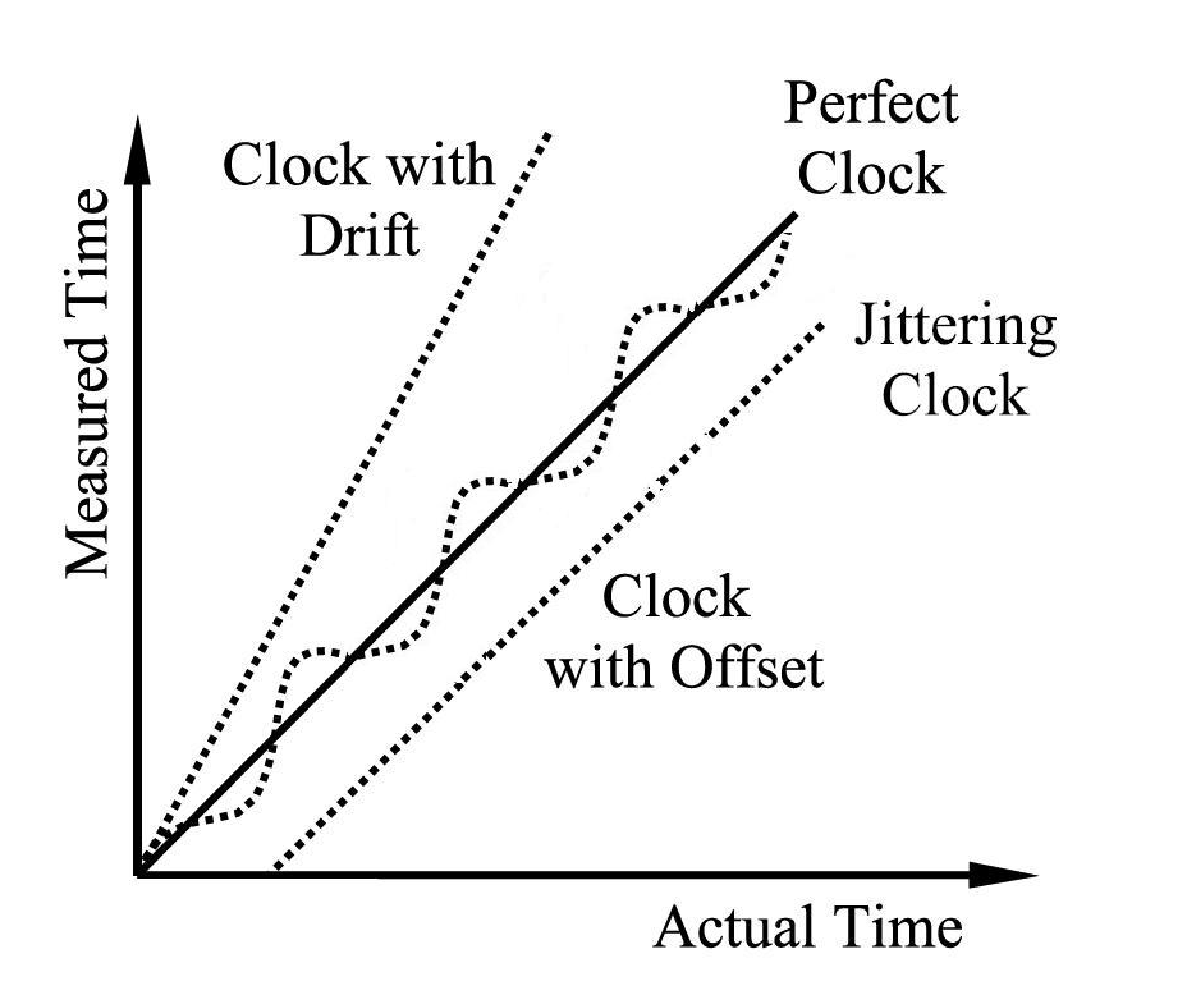
\includegraphics[width=0.35\textwidth]{actualvsmeasuredtime}
%\caption{Measured time versus real time}
%\label{fig:clocktimevsrealtime}
%\end{figure}
From the definition of frequency:
\begin{equation}
f = d\phi/dt \label{freq_defn} ,
\end{equation}
and integrating both sides over time,
 \begin{equation}
\phi =\int f(t)dt ,
 \end{equation}
where $f$ is frequency, $\phi$ is phase, and $t$ is time.\par
Thus, the clock time is described as
\begin{equation}
C(t) = \dfrac{1}{f_o}\int_{t_o}^{t} {f(\tau)d\tau} + C(t_o) ,
\label{clock}
\end{equation}
where $f(\tau)$ is the frequency of the clock, $f_o$ is the nominal frequency of the crystal oscillator
and $t_o$ is the start time of the node. \par The exact clock drift is hard to predict because it depends
on environmental influences but can be usually assumed that it doesn't exceed a maximum
 value $\rho$. % This means that it can be assumed$\cite{clockwhite}$
%\begin{equation}
%1-\rho \leq \dfrac{dC(t)}{dt} \leq 1+\rho ,
%\end{equation}
%where $\rho$ represents the maximum clock drift.
Note that different clocks have different maximum clock drift values $\rho$.\par The frequency of the clock is dependent on different
factors and can be given$\cite{clockwhite}$ as
\begin{equation}
f_i(t) = f_o + \Delta f + a(t-t_o) + \Delta
f_e(t) + \Delta f_n(t) \label{frequency}
\end{equation}
where $t_o$ = the start time of the clock, $a$ = aging factor, $f_o$ = nominal frequency,
 $\Delta f$ = calibration error, $\Delta f_n(t)$ = frequency instability (noise) term, $\Delta f_e(t)$ = frequency error which occurs due to outside factors like temperature and voltage instability. \par
From ($\ref{clock}$) and ($\ref{frequency}$),
\begin{equation}
C_i(t) - C_i(t_o) = \dfrac{1}{f_o} \int^{t}_{t_o}f_i(\tau)d\tau ,
\end{equation}
\begin{eqnarray*}
C_i(t) - C_i(t_o) & = & \dfrac{1}{f_o} \int^{t}_{t_o}{[f_o + \Delta f + a(\tau-t_o)  } \\
 &  & {} + \Delta f_e(\tau) + \Delta f_n(\tau)]d\tau ,
\label{fasika}
\end{eqnarray*}
\begin{eqnarray*}
C_i(t) & = & C_i(t_o) + (t-t_o) +\dfrac{\Delta f}{f_o}(t-t_o) \\
& & + \dfrac{a}{2f_o}(t-t_o)^2 + \dfrac{1}{f_o}\int^{t}_{t_o}{\Delta f_e(\tau)d\tau} +
\dfrac{1}{f_o}\int^{t}_{t_o}{\Delta f_n(\tau)d\tau} .
\end{eqnarray*}
A 32 kHz crystal clock $\cite{18,19}$  is used in the MyriaNode$\footnote{MyriaNode is the
 prototype sensor node which is built for the project MyriaNed.}$. Some notes to be considered in the model are:
\begin{itemize}
\item The amplitude of the short term variations due to noise $\Delta f_n(t)$ is small enough that they do not cause the clock to
accelerate or decelerate in a large amount in the long run.
\item Individual clock properties are assumed to be uncorrelated.
\item Clock parameters are normally distributed. The variances of the constants (initial time,
 initial frequency error, aging rate)$\cite{18,19}$ are all inputs to the model.
\item The spread in clock time grows almost linearly as a function of time, due to the dominance of the linear term in the clock drift equation.
\end{itemize}
\subsection{\textbf{Median algorithm and the setback}}
\par The Median algorithm is currently implemented in the MyriaNode. With the simplicity concerning
 the computational need, it is the best fit for WSN requirements discussed in the previous section.
The algorithm is described as follows:
\begin{enumerate}
\item Nodes broadcast packets.
\item Each receiver records the time that the packet is received according to the local clock.
\item Each receiver $i$ computes its phase error to any other node $j$ in the neighborhood as
\begin{equation}
\Delta t_{ij}^{(n)} = t_i^{(n)} - t_j^{(n)} ,\label{err}
\end{equation}
where $t_i$ is the wake-up time of node $i$ and $t_j$ is the wake-up
time of node $j$ at the $n^{th}$ period.
\item Receivers compute the offset, $\xi_i$, which is the median of the phase errors,
\begin{equation}
\xi_i^{(n)} = median(\Delta t_{ij}^{(n)}) , \forall j
\end{equation}
\item Receivers adjust their wake-up time by the computed offset value,
\begin{equation}
t_{i}^{(n+1)} = t_i^{(n)} + T_i^{(n)} - G\xi_i^{(n)},
\end{equation}
where $G$ is the gain factor.
\end{enumerate}
\begin{figure}[b]
\centering
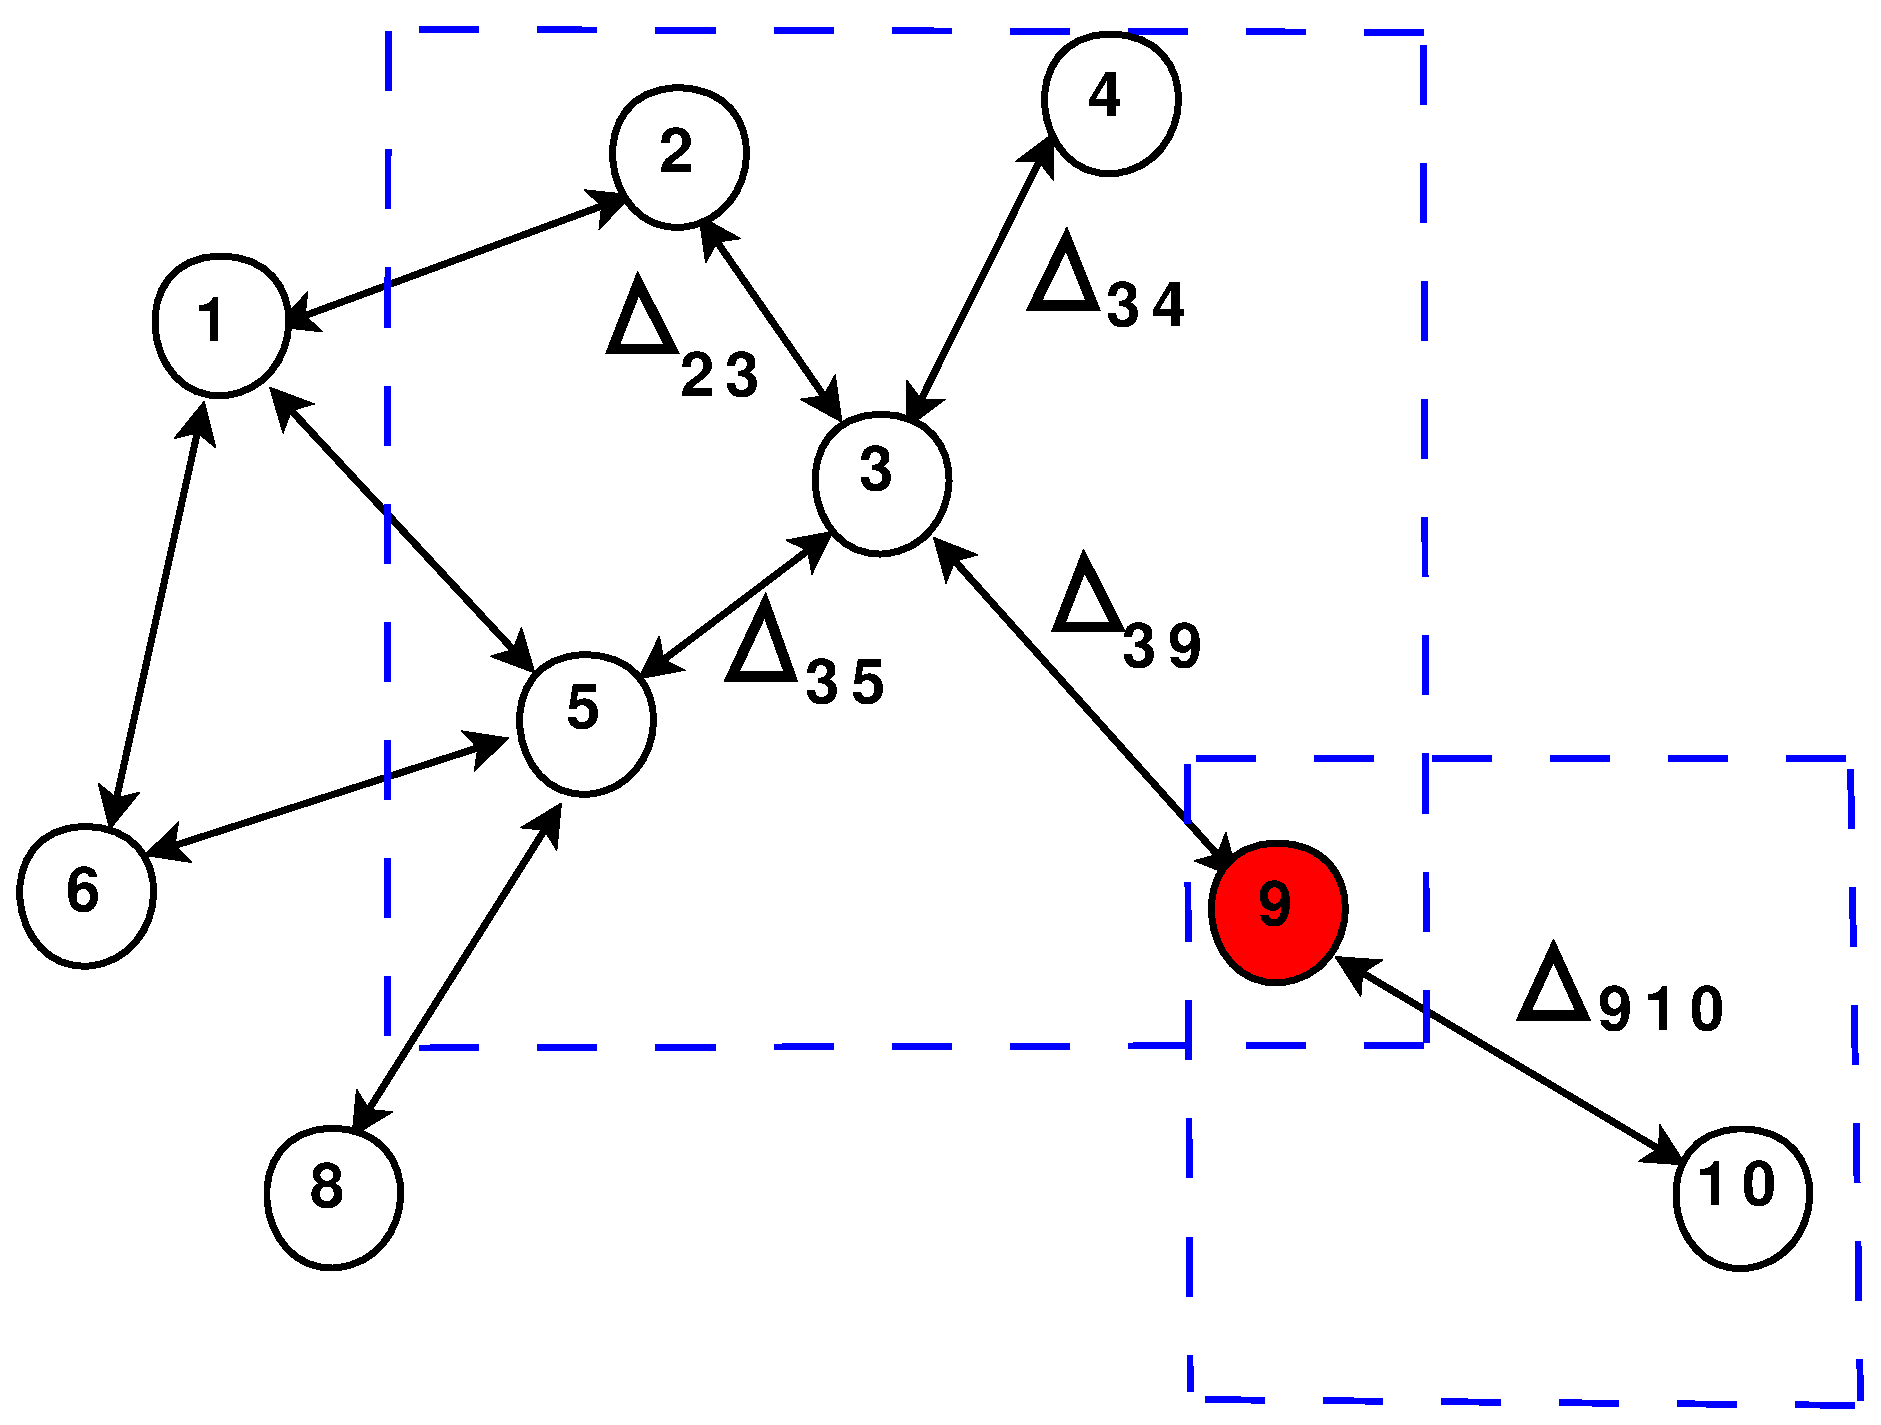
\includegraphics[width=0.4\textwidth]{node_field}
\caption{A WSN scenario} \label{wsn}
\end{figure}
By multiplying the median with a gain factor, $G\xi_i^{(n)}$, the output can be adjusted for better performance.
\par As per the application of Median, there are setbacks on its implementation. In some test-cases, the algorithm fails to converge or stays unsynchronized for a certain period of time.
\par A typical scenario is presented where the Median algorithm takes a longer time to achieve synchronization. In Figure $\ref{wsn}$, a distribution of nodes is shown. Node 10 joins  the stable network communication through Node 9. Assume Node 9 belongs to two broadcast domains, Node 3's and Node 10's. Thus, upon the application of the median algorithm, the node tends to adjust its wake-up time with the median of the phase errors from its neighbors, Node 3 and Node 10. Adjusting the wake-up time, the offset is
\begin{equation}
\xi_9 = median(\Delta t_{9,10} ,\Delta t_{9,3}).
\end{equation}
\begin{figure}
\centering
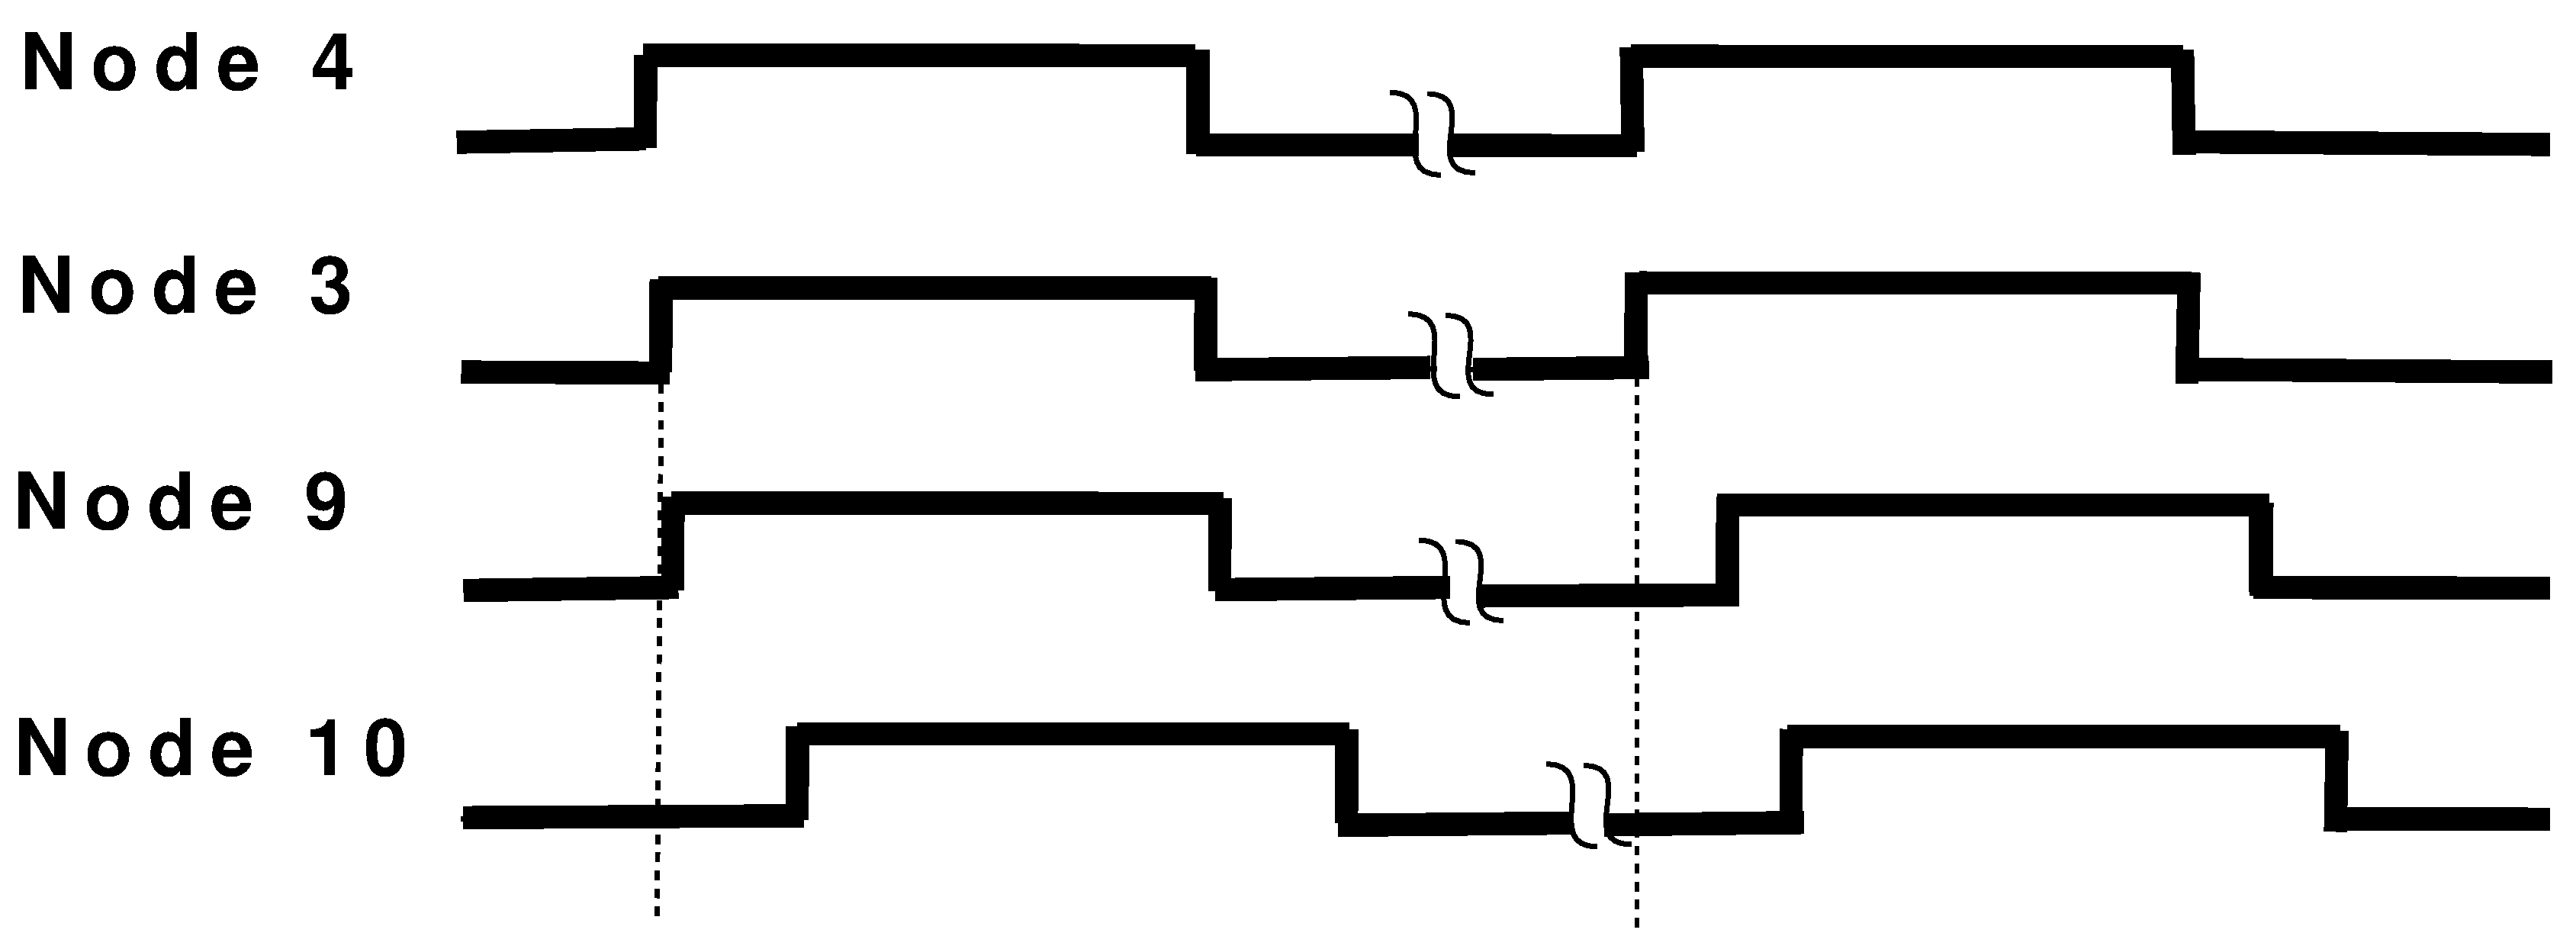
\includegraphics[width= 0.5\textwidth]{offsetpic}
\caption{Using median for phase error correction} \label{fasik}
\end{figure}
Being in synchronization with the other nodes, Node 9 will drift away from the network after its adjustment with Node 10. Therefore, it will take Node 9 more time to synchronize with the network again. Figure $\ref{fasik}$ shows the state of the network after the synchronization using the Median.
\par So, in order to address this problem, three algorithms are proposed in the next section to realize an energy-efficient, more precise and simple frame synchronization.
\section{\textbf{Synchronicity protocol}}
\subsection{\textbf{Synchronization frequency}}
%\textbf{Precise synchronization}: Precise synchronization is implemented when a node has already joined in the network, which repeatedly adjusts the diversion of its time slot reference caused by propagation delay and clock drift. \par
Decreasing the timing of the synchronization and executing the synchronization algorithms periodically reduces
the energy consumption of the WSN greatly. Thus, a synchronization period, $T_{sync}$, is defined as the period in which the network can stay synchronized without the application of the synchronization algorithm.
%\par A TDMA slot, $t_{slot}$, can be expressed in a
%number of clock cycles as
%\begin{equation}
%t_{slot} = kT ,
%\end{equation} where $T$ is the period of the frame in clock cycles and $k$ is a constant.
\par With a synchronization period $T_{sync}$ and the
maximum clock drift of a clock $\rho$ , the maximum time difference
between a sender and a receiver is
\begin{equation}
t_{diff} = 2\dfrac{T_{sync}}{T}\rho ,
\end{equation}
where $T$ is the period of the frame and the factor of $2$ reflects the worst case scenario where each
node's clock drifts in the opposite direction.\par
A time interval, guard time $t_{guard}$, is usually left vacant (i.e., during which no data is sent) on a transmission channel that can be used for synchronization and/or compensating for a signal distortion. In achieving frame synchronization in a TDMA scheduling, a guard time is given for a fault tolerance which is used to accommodate the phase errors, as shown in Figure $\ref{guardtime}$.
\begin{figure}[t]
\centering
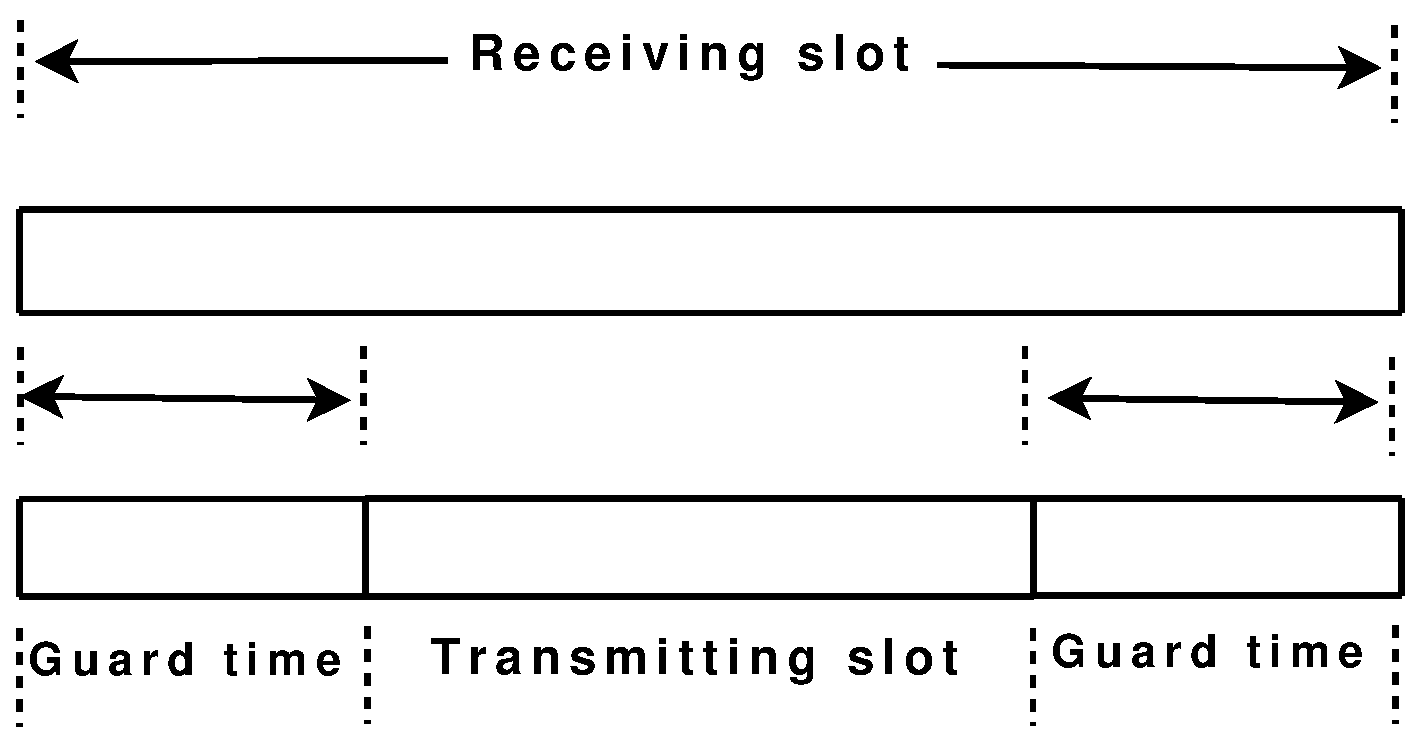
\includegraphics[width=2.5in]{guardtime}
\caption{Guard time of the nodes} \label{guardtime}
\end{figure}
Since the relative time difference between two nodes can be in two direction, the guard time needs to be twice $t_{diff}$,
\begin{equation}
t_{guard}= 2t_{diff} = 4\dfrac{T_{sync}}{T}\rho.
\end{equation}
At this end, the minimum duration for a time slot $t_{slot}$ is
\begin{equation}
t_{slot} \geq t_{guard} + T_{tx},
\end{equation}
where $T_{tx}$ is the time required to send a packet from one node to other.
\par Two nodes have a good communication link when they synchronize
their clocks at least once every $T$ that gives the following
relation,
\begin{equation}
\dfrac{T_{sync}}{T}\geq 1.
\end{equation}
To obtain the value of $T_{sync}$ for a particular system with a given duty cycle, the following equations are to be seen:
\begin{equation}
t_{guard} \geq 4\rho \dfrac{T_{sync}}{T}
\end{equation}
\begin{equation}
t_{slot} \geq t_{guard} + T_{tx}
\end{equation}
\begin{equation}
\dfrac{T_{sync}}{T} \geq 1.
\end{equation}
In general, there is a trade-off in determining $T_{sync}$: increasing $T_{sync}$ reduces the energy costs of synchronization, whereas decreasing the network performance.
\subsection{\textbf{Mathematical model}}
As part of the message, the nodes send the slot number which they
are transmitting to the neighbors. This information is used in
determining the time that the message is sent. Each message that is
sent within a slot is exactly received by a neighbor at a known
clock tick number
\begin{equation}
tick_{rx} = T_{tx}+ \dfrac{t_{guard}}{2} \label{tick}
\end{equation}
Whenever ($\ref{tick}$) is not satisfied, a phase error is observed. \par
The wake-up time of a node after $n$ periods of firings since it is turned on is
\begin{equation}
t_i^{(n)} = \sum_{n} T_i^{(n)} + t_{io},
\end{equation}
where  $T_i^{(n)}$ is the period of the crystal clock at the $n^{th}$ period which changes with time according to ($\ref{frequency}$) and $t_{io}$ is the initial start-up time of the node.\par
The difference in the wake-up time, ($\ref{err}$), of the nodes is therefore given by
\begin{eqnarray}
\Delta t_{ij} & = & \sum_{n}T_i^{(n)} + t_{io}- (\sum_{n}T_j^{(n)} +
t_{jo}) \\ &=& (\sum_{n}T_i^{(n)} - \sum_{n}T_j^{(n)}) +
(t_{io}-t_{jo}).
\end{eqnarray}
This phase error can be compensated by adjusting the next wake-up time
depending on the difference between the current wake-up time of the
node and its neighbors. Hence, the next wake-up time of the node is
dependent on the current wake-up time of its neighbors in relation
to its previous wake-up time,
\begin{equation}
t_i^{(n+1)} = t_i^{(n)} + T_i^{(n)} - \xi_i^{(n)} ,
\end{equation}
where $T_i$ is the period of the node's clock and $\xi_i$ is given
by
\begin{equation}
\xi_i = f(\Delta t_{ij}).
\end{equation}
The function $f$ is based on an algorithm which takes the wake-up
time differences between the node and its neighbors and determines
the optimal offset to be added to the next wake-up time of the node.
\par Three algorithms are proposed in the next subsections.
\subsubsection{\textbf{Weighted Measurements}}
One form of approach to tackle the dynamic behavior of a WSN is a
Weighted Measurements (WM) approach. Using this approach, different
weights are given to the different measurements. A weight is added to
increase the influence of the close by neighbors and ensure
faster synchronization. In addition to that, a new joining neighbor
can get synchronized with out disturbing the existing neighbors,
adjusting its time to the big swarm of nodes.\par
The offset is then
\begin{equation}
\xi_i^{(n)} = \sum_j{w_{ij}^{(n)}\Delta t_{ij}^{(n)}} ,
\end{equation}
where $\sum_j{w_{ij}^{(n)}= 1}$ and $w_{ij}$ is the weight factor
for the phase error, $\Delta t_{ij}$.
\par
The weighted adjustment is used to modify the next wake-up time of
the node,
\begin{eqnarray*}
t_i^{(n+1)} &=& t_i^{(n)} + T_i^{(n)} - \xi_i^{(n)} \\ &=& t_i^{(n)}
+ T_i^{(n)} - \sum_{j=0}^N{w_{ij}^{(n)}\Delta t_{ij}^{(n)}} \\ &=&
t_i^{(n)}+ T_i^{(n)} -
\sum_{j=0}^N{w_{ij}^{(n)}(t_i^{(n)}-t_j^{(n)})} \\ &=& T_i^{(n)} + \sum_{j=0}^N{w_{ij}^{(n)}t_j^{(n)}}.
\end{eqnarray*}
\par
The main task in this model is how to choose the weight factors
so that the stability of the network (time wise) is achieved faster. The weight is selected in such a way that the a node
joining a network should adjust its time with the network that it is
joining. After each measurement, a phase error is associated with
the weight  factor to which shows how far is the node concerning the
time that it drifted away from its neighbors.
\par \noindent In the selection of the weight factor, two steps are taken. \par \noindent
Firstly, each phase error $\Delta t_{ij}$ is associated with a value, $\delta_{ij}$. $\delta_{ij}$ is used to weigh how far the neighbor nodes has drifted. The $\delta$ values are calculated as:
\begin{equation}
\delta_{ij} = ae^{-b\Delta t_{ij}}.
\end{equation}
\begin{figure}[t]
\centering
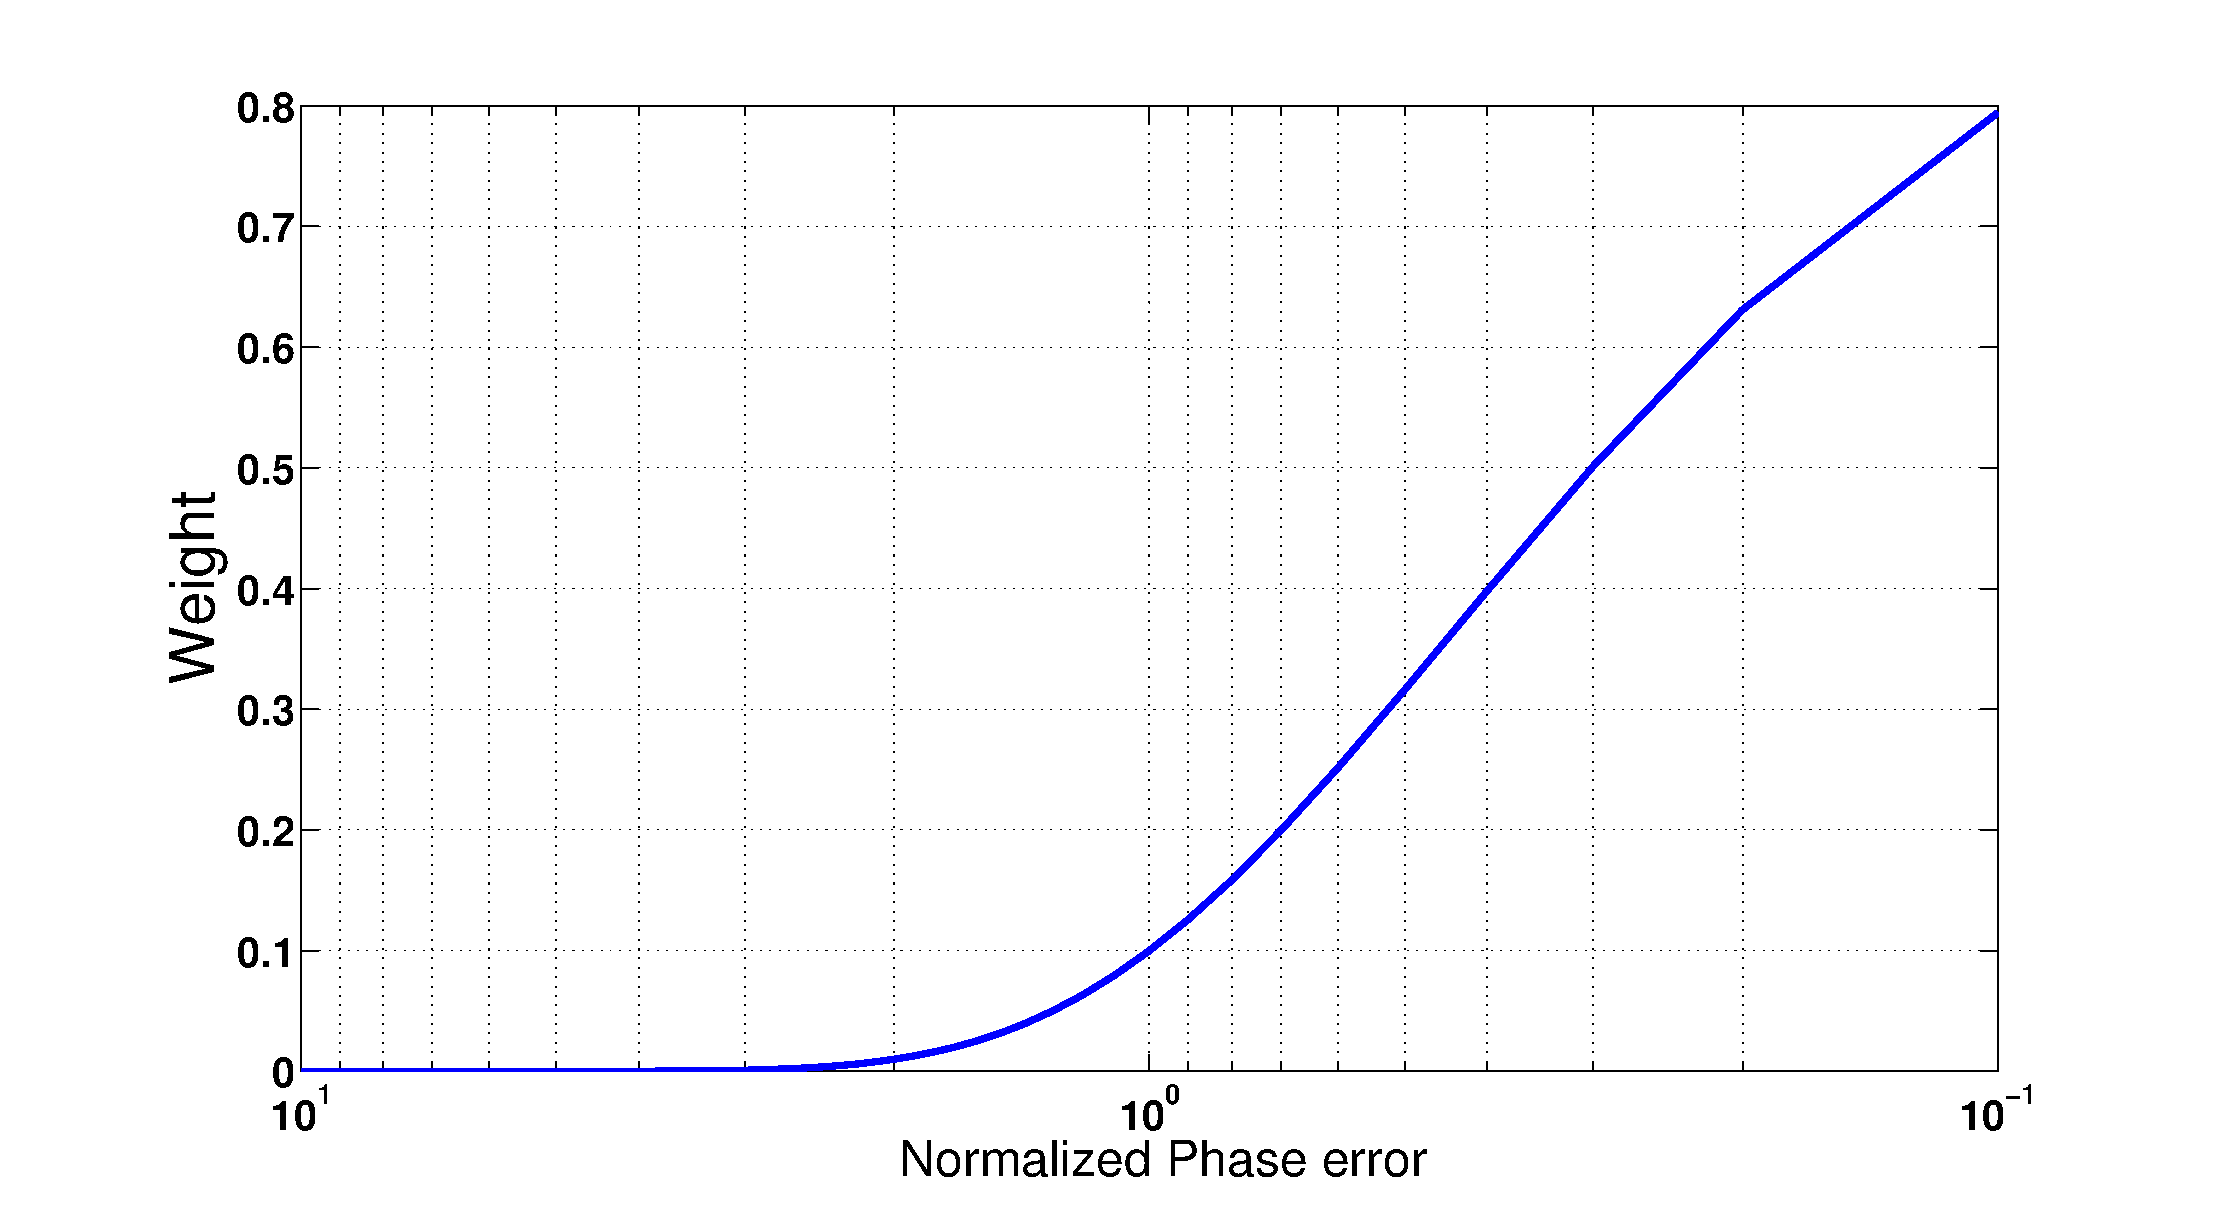
\includegraphics[width= 0.5\textwidth]{weightphase}
\caption{pre-weight factors for the phase error distribution}
\label{weight}
\end{figure} \noindent
The parameters $a$ and $b$ are selected using the initial conditions, $\delta_{ij}=0.1$ for $\Delta t_{ij}$ = $t_{guard}$ and $\delta_{ij}=1$ for $\Delta t_{ij}$ = 0. As shown in Figure $\ref{weight}$, the closer the phase error is to zero, the higher value of $\delta$ it is assigned. The assignment of high values to  small phase errors will decrease the time it takes to synchronize this node with the network.
\par \noindent
Secondly, the weight factor is calculated based on the distribution of the assigned values for each phase error. If all or most of the phase errors are small, this corresponds to the fact that the node has drifted away from most of the neighbors. Hence, the synchronization is made to adjust the nodes wake-up time towards the neighbors. \par \noindent
Hence, the weight factor is
\[w_{ij} = \left\{
\begin{array}{l l}
  1 - \delta_{ij},& \quad \mbox{if $mean(\delta_{ij}$) $<$ 0.5}\\
 \delta_{ij}, & \quad \mbox{if $mean(\delta_{ij}$) $>$ 0.5}\\ \end{array} \right. \]
where $mean$ is the average function.
The weight then moves towards the large phase errors if the node is a new-comer that wants to join the "already established" network.
\par
Therefore, in WM, the first step describes how the node has drifted away from its neighbors whereas the second step describes how the node is positioned in the network topology which surrounds it. Using the WM approach, a series of measurements will be used to estimate the next wake-up time of the node, giving less value/emphasis to the nodes which are out of reach from the neighboring nodes.
\subsubsection{\textbf{Least squares method}}
\par Least Squares (LS) is a method to fit a set of $n$ observations with a model of $m$ unknown parameters by minimizing the sum of the squares of the errors ("the residuals").
\par
It uses a set of $n$ data points, which are ($x_1$, $y_1$), ($x_2$, $y_2$),$\dots$,($x_n$, $y_n$), and a model function, $y= f(x, \beta)$, that in addition to the variable $x$ also depends on $m$ parameters($\beta_1,\beta_2,...,\beta_m$).
It is desired to find the vector $\beta$ of parameters such that the curve best fits the given data in the least squares, that is, the sum of squares
\begin{equation}
    S=\sum_{i=1}^{n}r_i^2 ,
\end{equation}
is minimized, where the residuals $r_i$ are given by
\begin{equation}
    r_i = y_i - f(x_i,\beta),
\end{equation}
for i=1,2,$\dots$, $n$.
\par
The minimum value of $S$ occurs when the gradient is zero. Hence, there are $m$ gradient equations to be solved where
\begin{equation}
    \dfrac{\partial S}{\partial \beta_j}=2\sum_i r_i\dfrac{\partial r_i}{\partial \beta_j}=0  \quad for \quad j=1,2...,m.
\end{equation}
In a non-linear system, the derivatives $\dfrac{\partial r_i}{\partial \beta_j}$ are functions of both the independent
variable and the parameters. These gradient equations do not have a closed solution. Instead, initial values must be chosen for the
parameters. Then, the parameters are refined iteratively, that is, the values are obtained by successive approximation,
\begin{equation}
    \beta_j^{p+1}=\beta^p_j+\Delta \beta_j.
\end{equation}
for $j=1,2...,m.$ Here, $p$ is an iteration number and the vector of increments, $\Delta \beta_j$, is the shift vector. At each iteration, the model is linearized by approximation to a first-order Taylor series expansion about $\beta^p$.
\begin{equation}
    f(x_i,\beta)\approx f(x_i,\beta^p) +\sum_j \dfrac{\partial f(x_i, \beta^p)}{\partial \beta_j} \left(\beta^p_j -\beta_j \right)
\end{equation}
\begin{equation}
 f(x_i,\beta) =f(x_i, \beta^p)+\sum_j J_{ij} \Delta\beta_j.
\end{equation}
The Jacobian, $J$, is a function of constants, the independent
variable and the parameters. So, it changes from one iteration to the
next. Thus, in terms of the linearized model,
\begin{equation}
\dfrac{\partial r_i}{\partial \beta_j}=-J_{ij}
\end{equation}
and the residuals are given by
\begin{equation}
    r_i=\Delta y_i- \sum_{j=1}^{m} J_{ij}\Delta\beta_j,
\end{equation}
where
\begin{equation}
 \Delta y_i=y_i- f(x_i, \beta^p).
\end{equation}
Substituting these expressions into the gradient equations and
equating to $0$, the resulting system of equations can be
represented as a matrix notation as
\begin{equation}
    \left(J^TJ\right)\Delta  \beta=J^T\Delta y.
\end{equation}
\textbf{Model design} \par
As the algorithm is decentralized, the next wake-up time of the node depends on
the current phase errors that it has with the other nodes. The distribution of the phase error is the crucial factor in deciding the type of curve to fit in. The phase errors shows how many time units that the neighbor node is out of touch with the node in focus. The larger the phase error is, the more out-of-sync the node is.\par
The set of data are the measured phase errors of the node with its neighbors.
In order to meet the demand of adjusting the time offset and stabilize the network, the logarithmic curve with the model
\begin{equation}
 f(x_i,\beta)= \beta _1 + \beta_2log(x_i),
\end{equation}
is chosen. A logarithmic function can be used to represent the
distribution of the phase errors in the neighborhood, as shown in
Figure $\ref{curvefit}$. In the figure, the neighborhood is taken to
have 50 nodes. Hence, the maximum phase error between the node and
its neighbors i.e. upper bound is taken to be the guard time of the
node, $t_{guard}$. Fitting the curve, the node will be synchronized
with its neighbors. Normalized phase error values tend to be small
and follow a curve in such away that the maximum value of the phase
error should not be greater than the guard time.
\begin{figure}
\centering
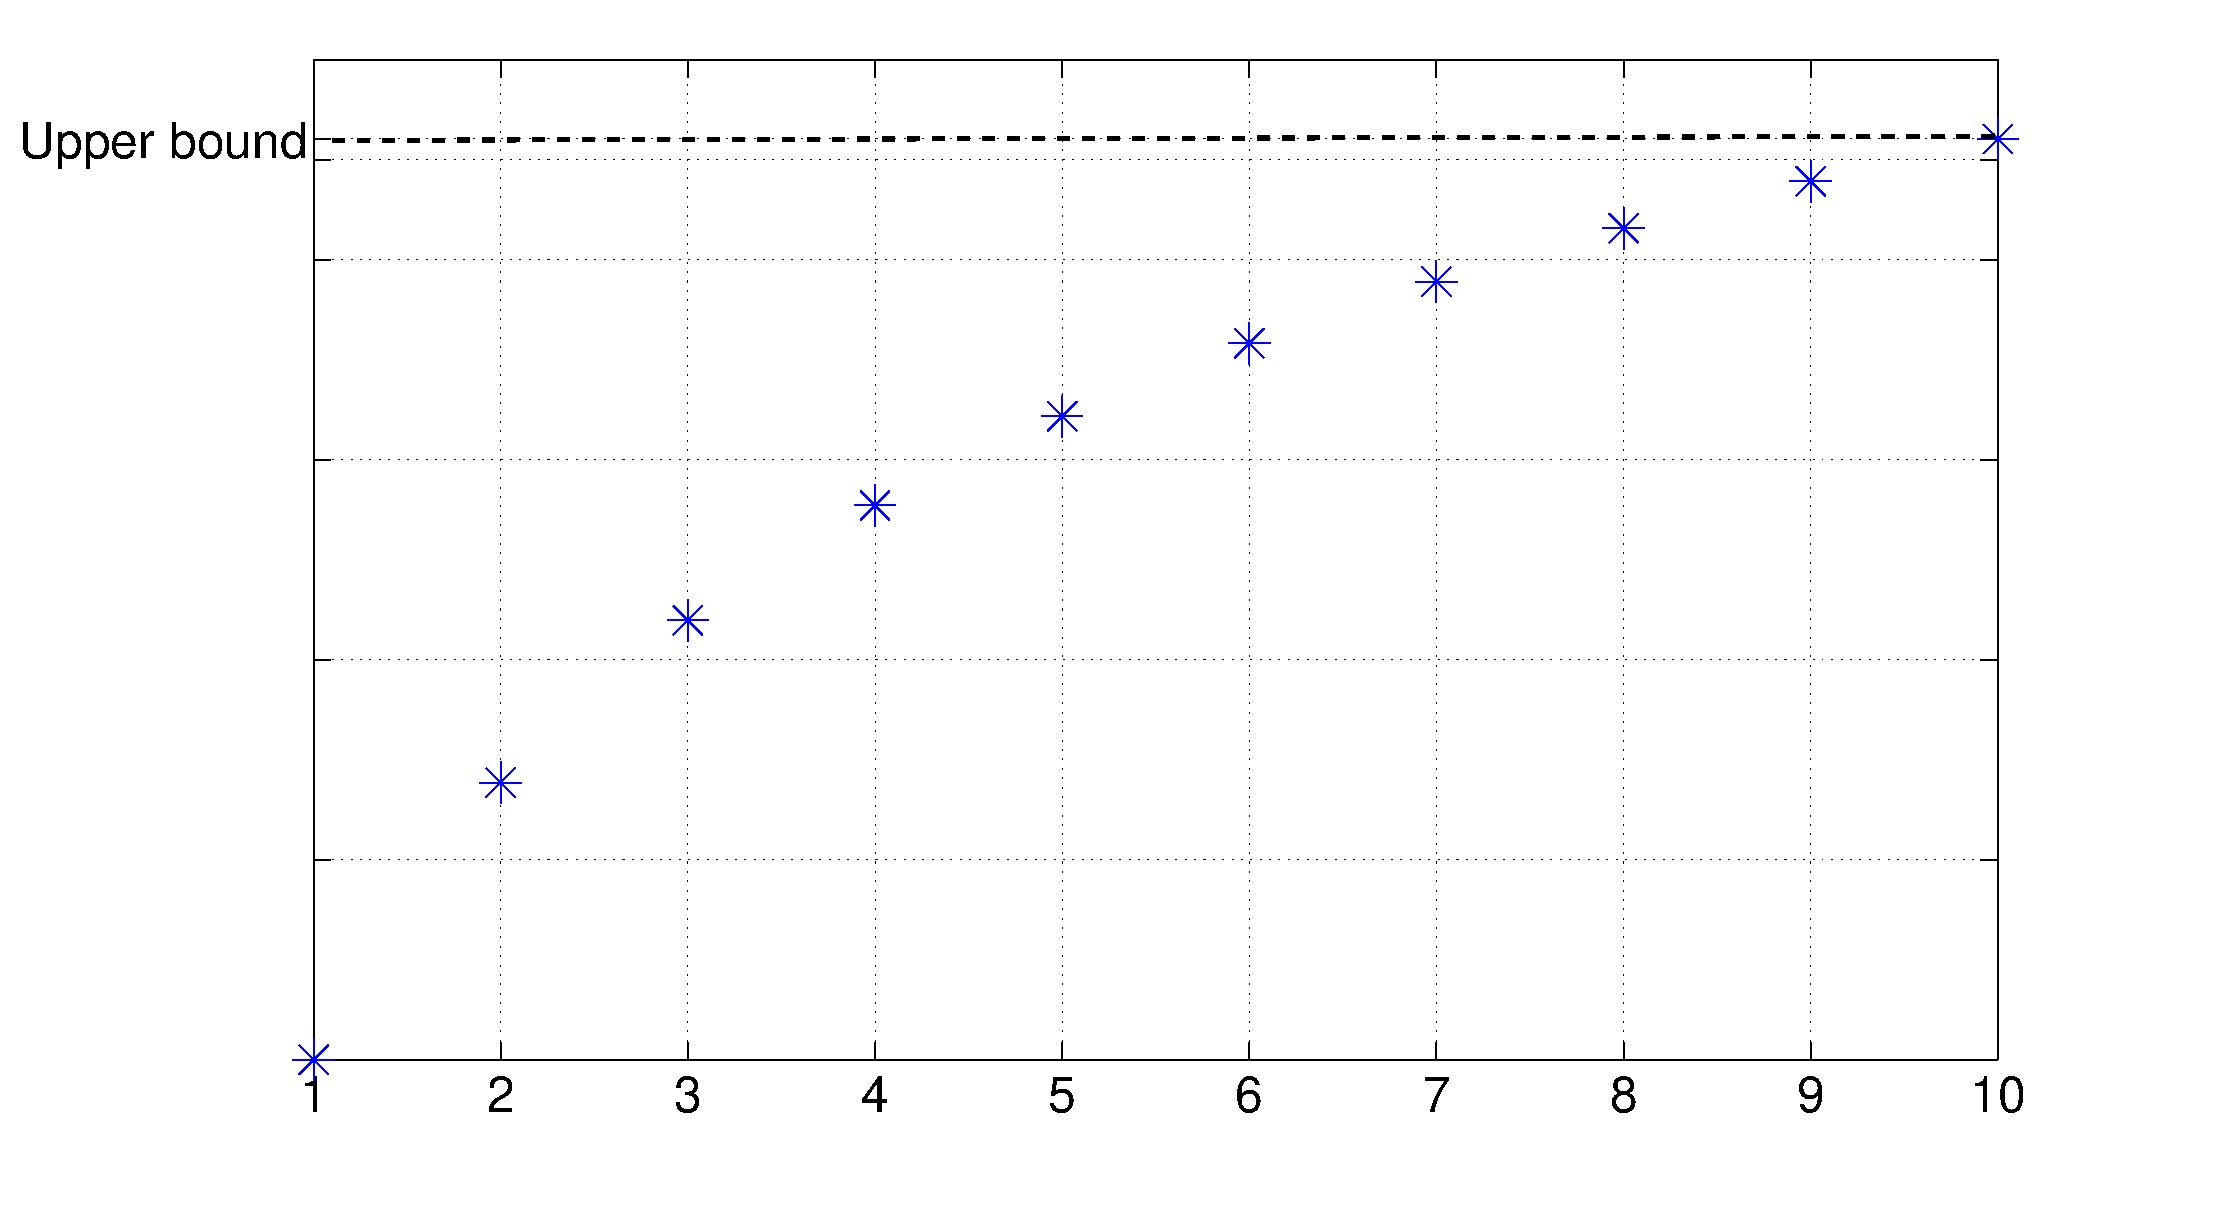
\includegraphics[width=0.5\textwidth]{curvefit}
\caption{Curve fitting using logarithmic function} \label{curvefit}
\end{figure}
\par
The initial values of the parameters $\beta_1$ and $\beta_2$ are
estimated using the state of a synchronized network taking into
account. As each measurement arrives from the neighbors, the
parameters are calculated in such a way that the measurement error
from a pre-determined offset value is reduced. This ensures that the
offset to be added in the next wake-up time doesn't diverge in a
large amount from the predicted value.
\subsubsection{\textbf{Discrete time kalman filter for synchronization}}
The kalman filter$\cite{kalm}$ estimates a process by using a form
of feedback control. It estimates the process state at some time and
then obtains feedback in the form of (noisy) measurements. As such,
the equations for the Kalman filter fall into two groups: time
update equations and measurement update equations. The time update
equations are responsible for projecting forward (in time) the
current state and error covariance estimates to obtain a priori
estimates for the next time step.
\par
The kalman filter addresses the general problem of trying to
estimate the state $x \in R$ of a discrete-time controlled process that is
governed by the linear stochastic difference equation
\begin{equation}
 x_k = Ax_{k-1} + Bu_k + w_{k-1} , \label{mainkal}
\end{equation}
with a measurement $z \in R$ that is
\begin{equation}
 z_k = Hx_k + v_k. \label{meakal}
\end{equation}
The random variables $w_k$ and $v_k$ represent the process and
measurement noise respectively. They are assumed to be
independent of each other, white, and with normal probability
distributions
\begin{equation}
 p(w) \approx N(0,Q),
\end{equation}
\begin{equation}
 p(v) \approx N(0,R).
\end{equation}
The $n\ x\ n$ matrix $A$ in ($\ref{mainkal}$) relates the state at
the previous time step $k-1$ to the state at the current step $k$,
in the absence of either a driving function or process noise. Note
that in practice $A$ might change with each time step, but here we
assume it is constant. The n × l matrix $B$ relates the optional
control input $u \in R$ to the state $x$. The $m\ x\ n$ matrix $H$
in $\ref{meakal}$ the relates the state to the measurement $z_k$. In
practice, $H$ might change with each time step or measurement, but
here we assume it is constant.
\par
We define $\tilde x_k^- \in R$ to be our a priori state estimate at
step k given knowledge of the process prior to step $k$, and $\tilde
x_k \in R$ to be our a posteriori state estimate at step $k$ given
measurement $z_k$. Hence, a priori and a posteriori estimate errors
are defined as
\begin{equation}
e_k^- = x_k – \tilde x_k^- ,
\end{equation}
\begin{equation}
e_k =  x_k – \tilde x_k.
\end{equation}
The a priori estimate error covariance is then
\begin{equation}
P_k^- = E[ e_k^- e_k^{-T} ],
\end{equation}
and the a posteriori estimate error covariance is
\begin{equation}
P_k = E[e_k e_k^T].
\end{equation}
With the initial estimates of $x_{k-1}$ and $P_{k-1}$, the predictor equations are
\begin{equation}
x_k = Hx_{k-1} + Bu_k,
\end{equation}
\begin{equation}
P_k = HP_{k-1}H^T + Q.
\end{equation}
The measurement update equations are responsible for the feedbacks
i.e. for incorporating a new measurement into the a priori estimate
to obtain an improved a posteriori estimate.
\begin{equation}
K_k = P_kH^T(HP_kH^T + R)^{-1} \label{kalmangain}
\end{equation}
\begin{equation}
x_k = x_k + K_k(z_k - Hx_x)
\end{equation}
\begin{equation}
P_k = (I-K_kH)P_k.
\end{equation}
The matrix K in ($\ref{kalmangain}$) is
chosen to be the gain or blending factor that minimizes the
posteriori error covariance. Taking the derivative of the trace of
the resulting derivative with respect to K, setting that result equal to zero, and
then solving for K provides
\begin{equation}
K_k = P_kH^{T}(HP_kH^{T} + R)^{-1}
\end{equation}
\begin{equation}
K_k = \dfrac{P_kH^T}{HP_kH^T + R}. \label{gain}
\end{equation}
Looking at ($\ref{gain}$), it is seen that as the measurement error
covariance $R$ approaches zero, the gain K weights the residual more
heavily. Specifically,
\begin{equation}
\mathop {\lim }\limits_{R_k \to 0 } {K_k} = H^{-1}.
\end{equation}
On the other hand, as the a priori estimate error covariance $P_k$
approaches zero, the gain K weights the residual less heavily.
Specifically,
\begin{equation}
\mathop {\lim }\limits_{P_k \to 0 } {K_k} = 0.
\end{equation}
The time update equations can also be thought of as predictor
equations, while the measurement update equations can be thought of
as corrector equations.
\par
The update equation is
\begin{equation}
\tilde x_k = \tilde x_k + K(z_k-H\tilde x_k).
\label{updatekalman}
\end{equation}
The difference $z_k - H\tilde x_k$ in ($\ref{updatekalman}$) is the residual. The residual reflects the discrepancy between the predicted measurement $H\tilde x_k$ and the actual measurement $z_k$. A residual of zero means that the two are in complete agreement. \par \noindent
\textbf{Filter design} \par
The transition matrix $A$ plays an important role in achieving
the proper synchronization. It indicates how fast/slow the next wake up time should be compared
to it's previous value and/or neighbors. The initial estimates of $x$ and $P$ are selected from the
previous firing time of the node, one period earlier. This ensures that the nodes are on the same track as the previous time, since the neighbors remain the same with some exception of mobility and interference. $H$ is a factor used to compare the predicted value to the measured value. \par
In the filter design, the covariance matrices $R$ and $Q$ have a significant
role in the overall implementation of the algorithm. $R$ represents how
 the measurements are valued to affect the outcome and $Q$
sends a signal as to how the estimated value is weighed.
\section{\textbf{Results and Discussion}}
\subsection{\textbf{Simulation setup}}
%In the simulation, a Discrete Event Simulator (DES) is used. A DES will break down a simulation into discrete chunks.
%Every event will occur at some countable time moment and will be given in chronological order. The
%advantage of this distinction is two-fold. First, simulations will
%not be dependant on some real-time clock. Second, events can be
%isolated to perform certain measurements.
%\par
%One such DES is MiXiM$\footnote{MiXiM (Mixed Simulator) is a
%simulation framework for wireless and mobile networks using the
%OMNeT++ $\cite{omnet}$ simulation engine. It is a collaborative
%project between TU Berlin, TU Delft and Universitaet Paderborn.}$.
%It provides a component architecture for models. Components are
%programmed in C++, then assembled into larger components and models
%using a high-level language. Octave$\footnote{Octave is a free
%program for performing numerical computations which is mostly\dfrac{}{}
%compatible with MATLAB. It is part of the GNU project.}$ is used for
%interpretation of the data from the network simulator.
The simulation parameters are presented in the following table.
\begin{center}
    \begin{tabular}{ | l | l |}
    \hline
    Duration time frame & 1s \\ \hline
    Number of slots &  10 \\ \hline
%    Attenuation constant & 2.5 \\ \hline
    Data rate &  2Mbps \\ \hline
    \end{tabular}
\end{center}
Nodes communicate by broadcasting. The start up time of the nodes is
gaussian distributed random variable, $t_{io}$. The nodes are
positioned uniformly across the simulation area at the start. The
proposed algorithms are KF, M, WM, LS which represent Kalman Filter,
Median, Weighted Measurments and Least Squares respectively. A clock
cycle is represented here as $clk$ which shows the resolution of the
quartz crystal clock. The synchronization error is defined as the
maximum difference between the wakeup time of the nodes in the
neighborhood. The simulation is conducted in different scenarios and
some test case results are presented here for discussion.
% \par The simulation is conducted 100 times to counter the effect of randomness introduced in the simulation.
\subsection{\textbf{Simulation results}}
\begin{figure*}
\centerline{
\subfloat[Number of Nodes - 20]{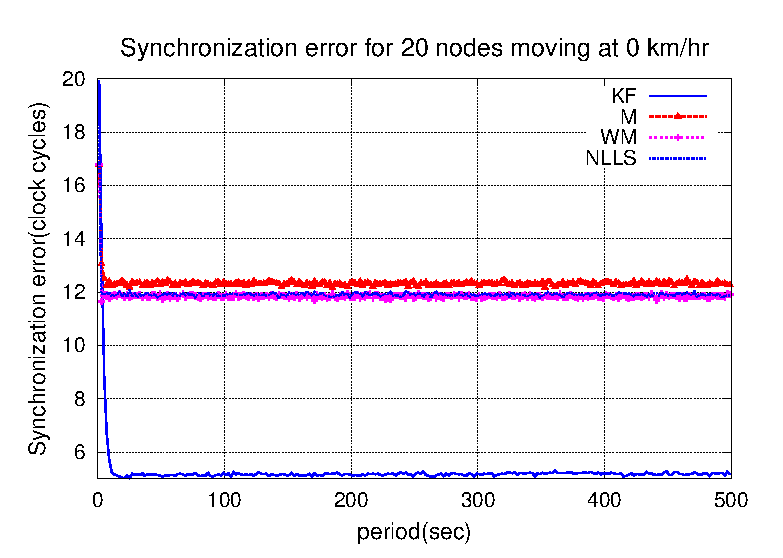
\includegraphics[width=0.5\textwidth]{16output-s0}
\label{16output0}}
\hfil
\subfloat[Number of Nodes - 50]{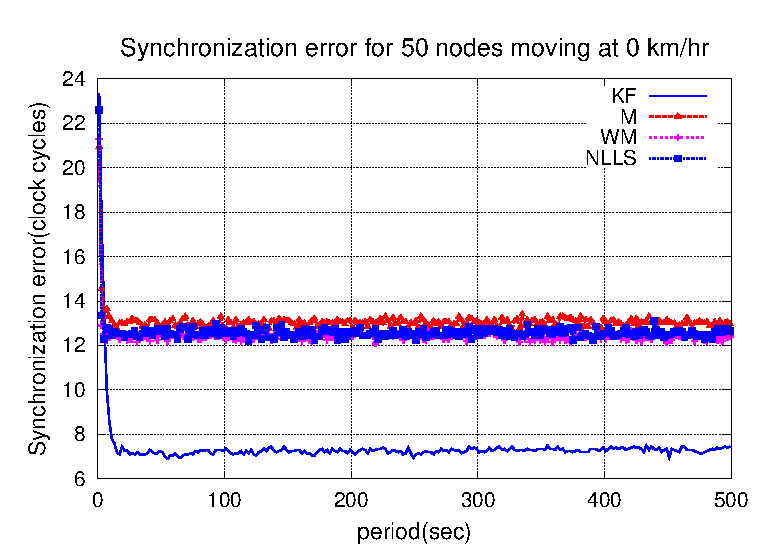
\includegraphics[width=0.5\textwidth]{50output-s0}
\label{50output0}}}
\caption{Simulation results for Static Nodes }
\label{static}
\end{figure*}
\subsubsection{\textbf{Case I}} 
In the first set of simulations, the synchronization error is simulated for the nodes which are static, hence no effect of mobility.
\par
Figure $\ref{16output0}$ shows the synchronization error for $20$
nodes operating in a static environment. The algorithms achieve a
stable synchronization. As LS and WM has the same effect as the
Median in case of stable network, the performance of both algorithms
is similar with that of Median. Without the dynamic nature of the
network, both tend to equal the average of the phase errors. KF has
the best performacesince correcting the phase errors involves
predict and update which results in better precision. \par
Figure $\ref{50output0}$ is the result of a simulation for $50$
nodes. The synchronization error in general increases as the number
of nodes increases. Comparing the individual algorithms, KF has the best
precision whereas LS and WM have a better performance
each than the Median. Median results in a lower performance on average.
\subsubsection{\textbf{Case II}}
\begin{figure*}
\centerline{
\subfloat[Speed - 6km/hr]{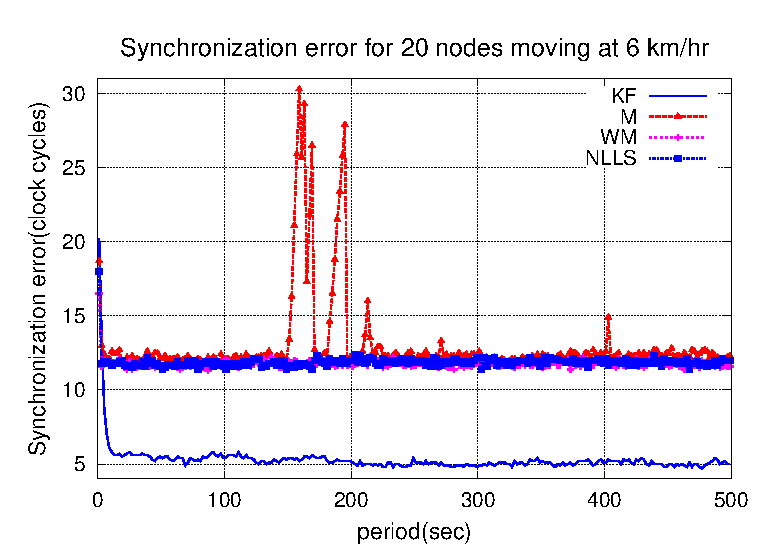
\includegraphics[width=0.5\textwidth]{16output-s6}
\label{16output6}} \hfil \subfloat[Speed -
20km/hr]{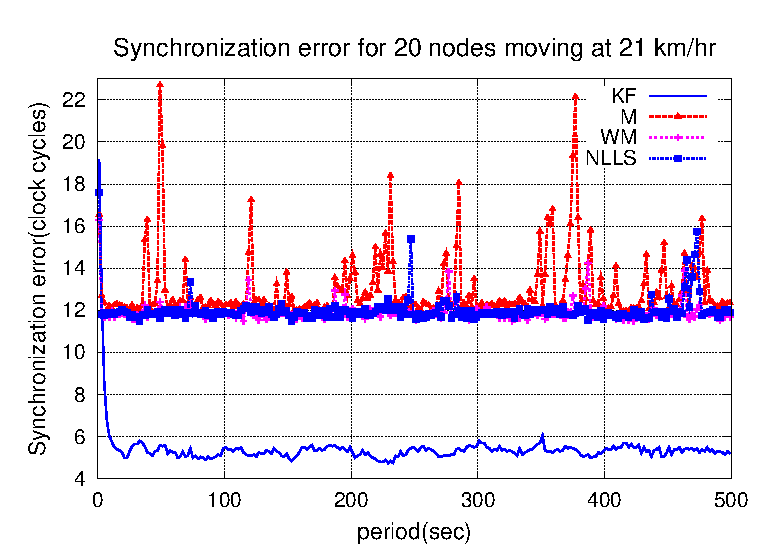
\includegraphics[width=0.5\textwidth]{16output-s20}
\label{16output20}}} \caption{Simulation results for 20 Nodes}
\label{16output}
\end{figure*}
In second set of simulations, the mobility of the nodes is taken into account. Here, the number of the nodes is taken to be $20$. The simulations are conducted for different speeds, at average speeds of $6km/hr$ and $20km/hr$. The chosen speeds emulate the speed of a walking man and an average speed of a slowly moving vehicle.
\par
In second set of simulations, the mobility of the nodes is taken
into account. Here, the number of the nodes is taken to be $20$. The
simulations are conducted for different speeds, at average speeds of
$6km/hr$ and $20km/hr$. The chosen speeds emulate the speed of a
walking man and an average speed of a slowly moving vehicle.
\par
Figure $\ref{16output6}$ shows 20 nodes with a speed which is an
gaussian random variable with mean $6km/hr$ and standard deviation
of 1$km/hr$. WM and LS show a better tolerance to dynamic networks
due to the algorthms capapbilty to synchronize towards a more stable
network. LS has also a better tolerance with less value given for
large phase errors. Hence, WM and LS perform better concerning the
synchronization of the frame than the Median.  Median algorithm has
a disruptions which made the network out-of-synchronization,
resulting in high synchronization errors at times. This occurs due
to the mobility of the nodes which disrupts the stability networks
as it tries to compute the median of the phase errors, as indicated
in Secton II. KF outperforms all due to its dynamic and recursive nature.
\par
The speed of the nodes is changed to a random variable with mean
$20km/hr$ and standard deviation $1km/hr$. The simulation results
are presented in Figure $\ref{16output20}$. KF performs the best
showing that the algorithm is stable in dynamic networks. WM and LS
perform good when it comes to stability. As the dynamics of the
networks increases, Median becomes more unstable and exhibits large
synchronization error. LS and WM have a stable performance when the
network becomes dynamic with constantly changing connection between
the nodes.
\par
The relative comparison of the algorithms performance improvement
with the Median is shown in Figure $\ref{16output-error}$ for nodes
moving at $20km/hr$. WM and LS perform, on average, $6-8\%$ better
than Median, but with more tolerance in handling the disruptions.
The best performer, KF, has on average $60\%$ better performance
than the Median one.
%\begin{figure}
%\centering 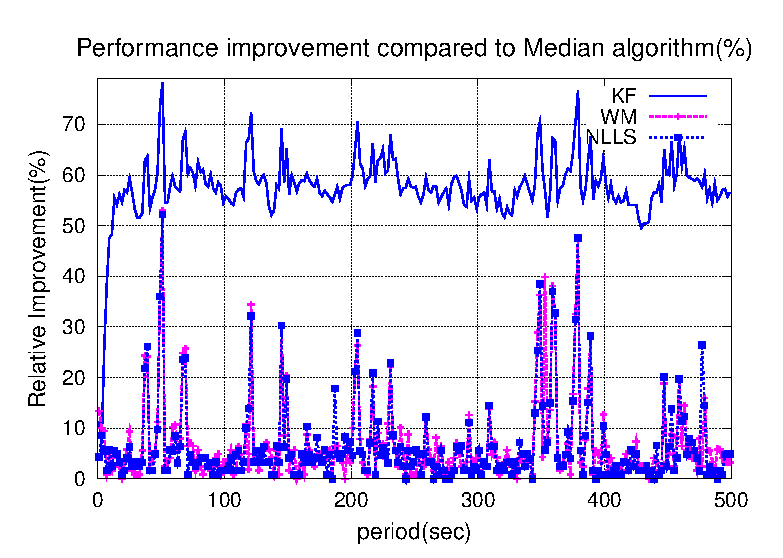
\includegraphics[width=0.5\textwidth]{16output-error}
%\caption{Relative error of the algorithms with respect to Median for 20 nodes}
%\label{16output-error}
%\end{figure}
\begin{figure*}
\centerline{ \subfloat[for 20 nodes]{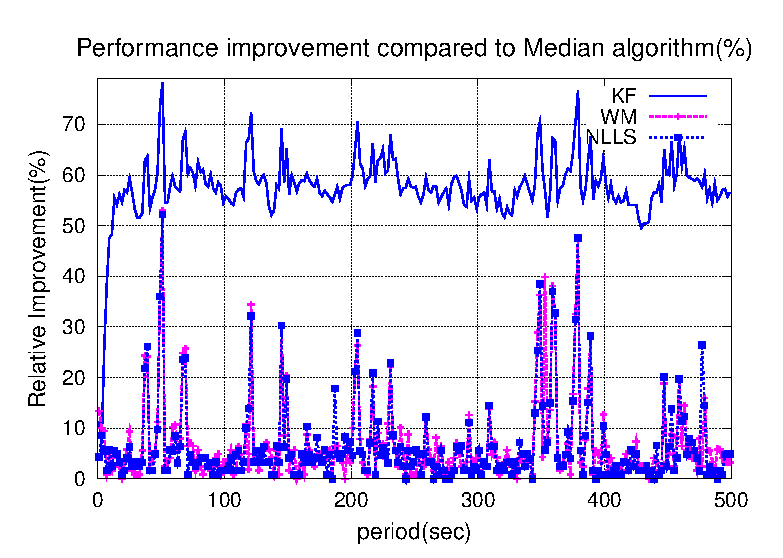
\includegraphics[width=0.5\textwidth]{16output-error}
\label{16output-error}} \hfil \subfloat[for 50 nodes]{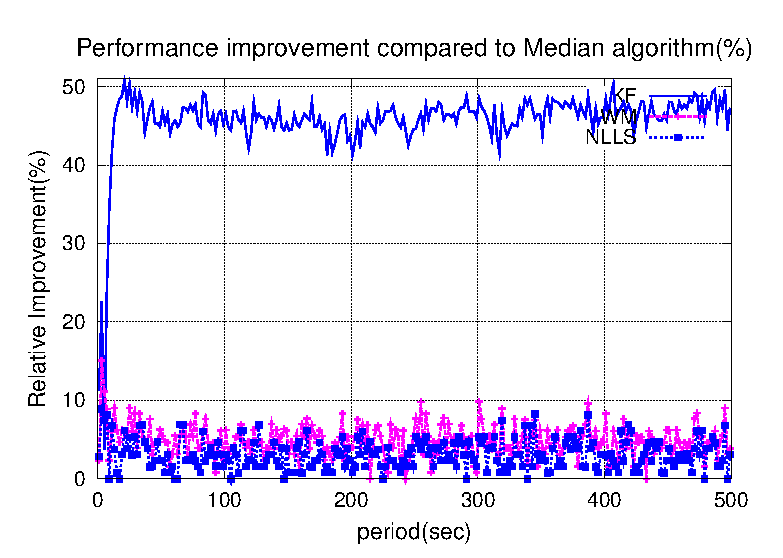
\includegraphics[width=0.5\textwidth]{50output-error}
\label{50output-error}}} \caption{Relative error of the algorithms with respect to Median}
\label{error}
\end{figure*}
\subsubsection{\textbf{Case III}}
\begin{figure*}
\centerline{ \subfloat[Speed -
5km/hr]{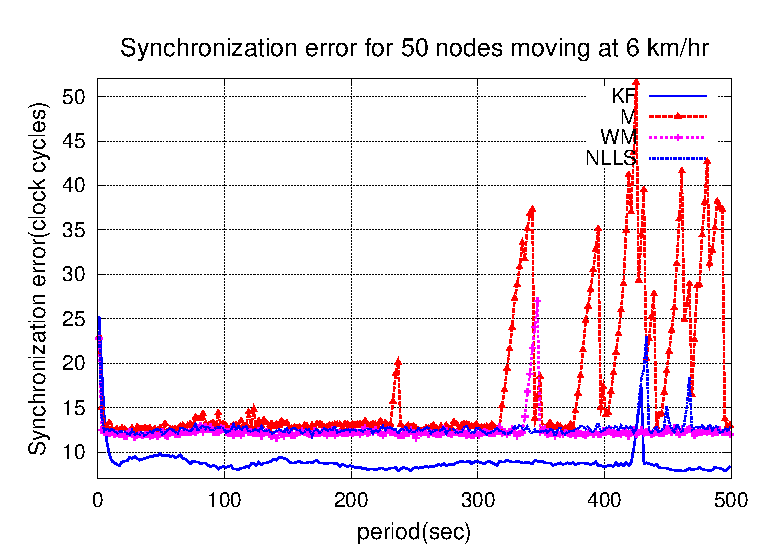
\includegraphics[width=0.5\textwidth]{50output-s6}
\label{50output6}} \hfil \subfloat[Speed -
20km/hr]{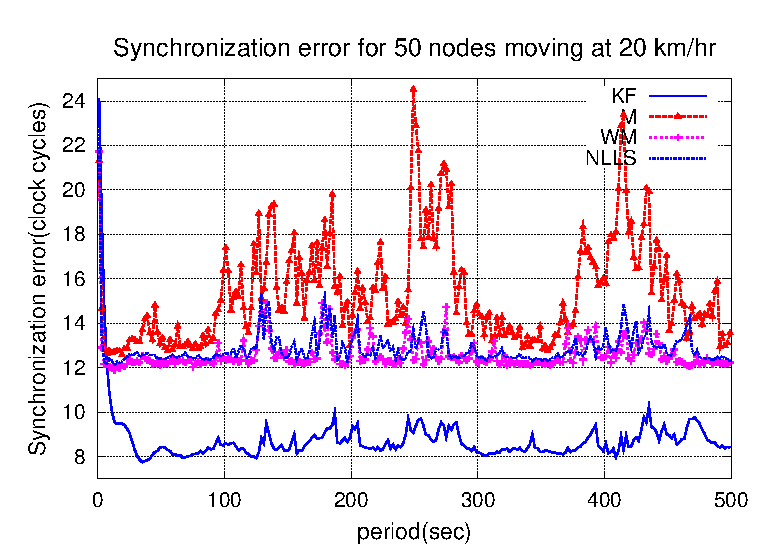
\includegraphics[width=0.5\textwidth]{50output-s20}
\label{50output20}}} \caption{Simulation results for 50 Nodes}
\label{50output}
\end{figure*}
In this set of simulations, the number of the nodes is increased, to
$50$. With slowly moving nodes ($6km/hr$), the results are shown in
Figure $\ref{50output6}$. Large disruptions occur when using Median
due to nodes moving slowly in the surrounding (leave the network and
join again after some time), resulting in a larger drift with
neighbors before getting back to the network. LS and WM perform
better when it comes to stability, as out-of-sync nodes are forced
to join the stable network. KF has the best preformance, both in
precision and stability. 
\par
With a speed of $20km/hr$, the simulation results are presented in Figure $\ref{50output20}$. As the speed increases, the instability
on the synchronization of the nodes also increases, which makes the Median more prone to high synchronization errors. WM has better
tolerance towards mobility of the nodes, whereas the LS does well regarding stability. KF has the best precision out of all. As the
speed increases, the precision of the synchronization increases too since faster speed results in faster synchronization within the network.
\par
For the set of nodes with a higher speed , a relative comparison is made to see the performance of the nodes with the Median algorithm. The Median algorithm is shown to perform the worst in this case. There are a lot of disruptions in the network, making it more unstable whereas the other algorithms adapt to the changes faster. Figure $\ref{50output-error}$ shows that KF performs the best against Median algorithm, $45\%$. WM and LS perform well against Median too, $20\%$ on average. It has been shown that the median is prone to error in case of high dynamics in the network.\par 
The Kalman filter has a better precision and stability than the rest whereas WM and LS has a better tolerance to a dynamic network.
\subsection{\textbf{Measurements concerning the energy consumption}}\noindent
%\begin{figure}[b]
%\centering
%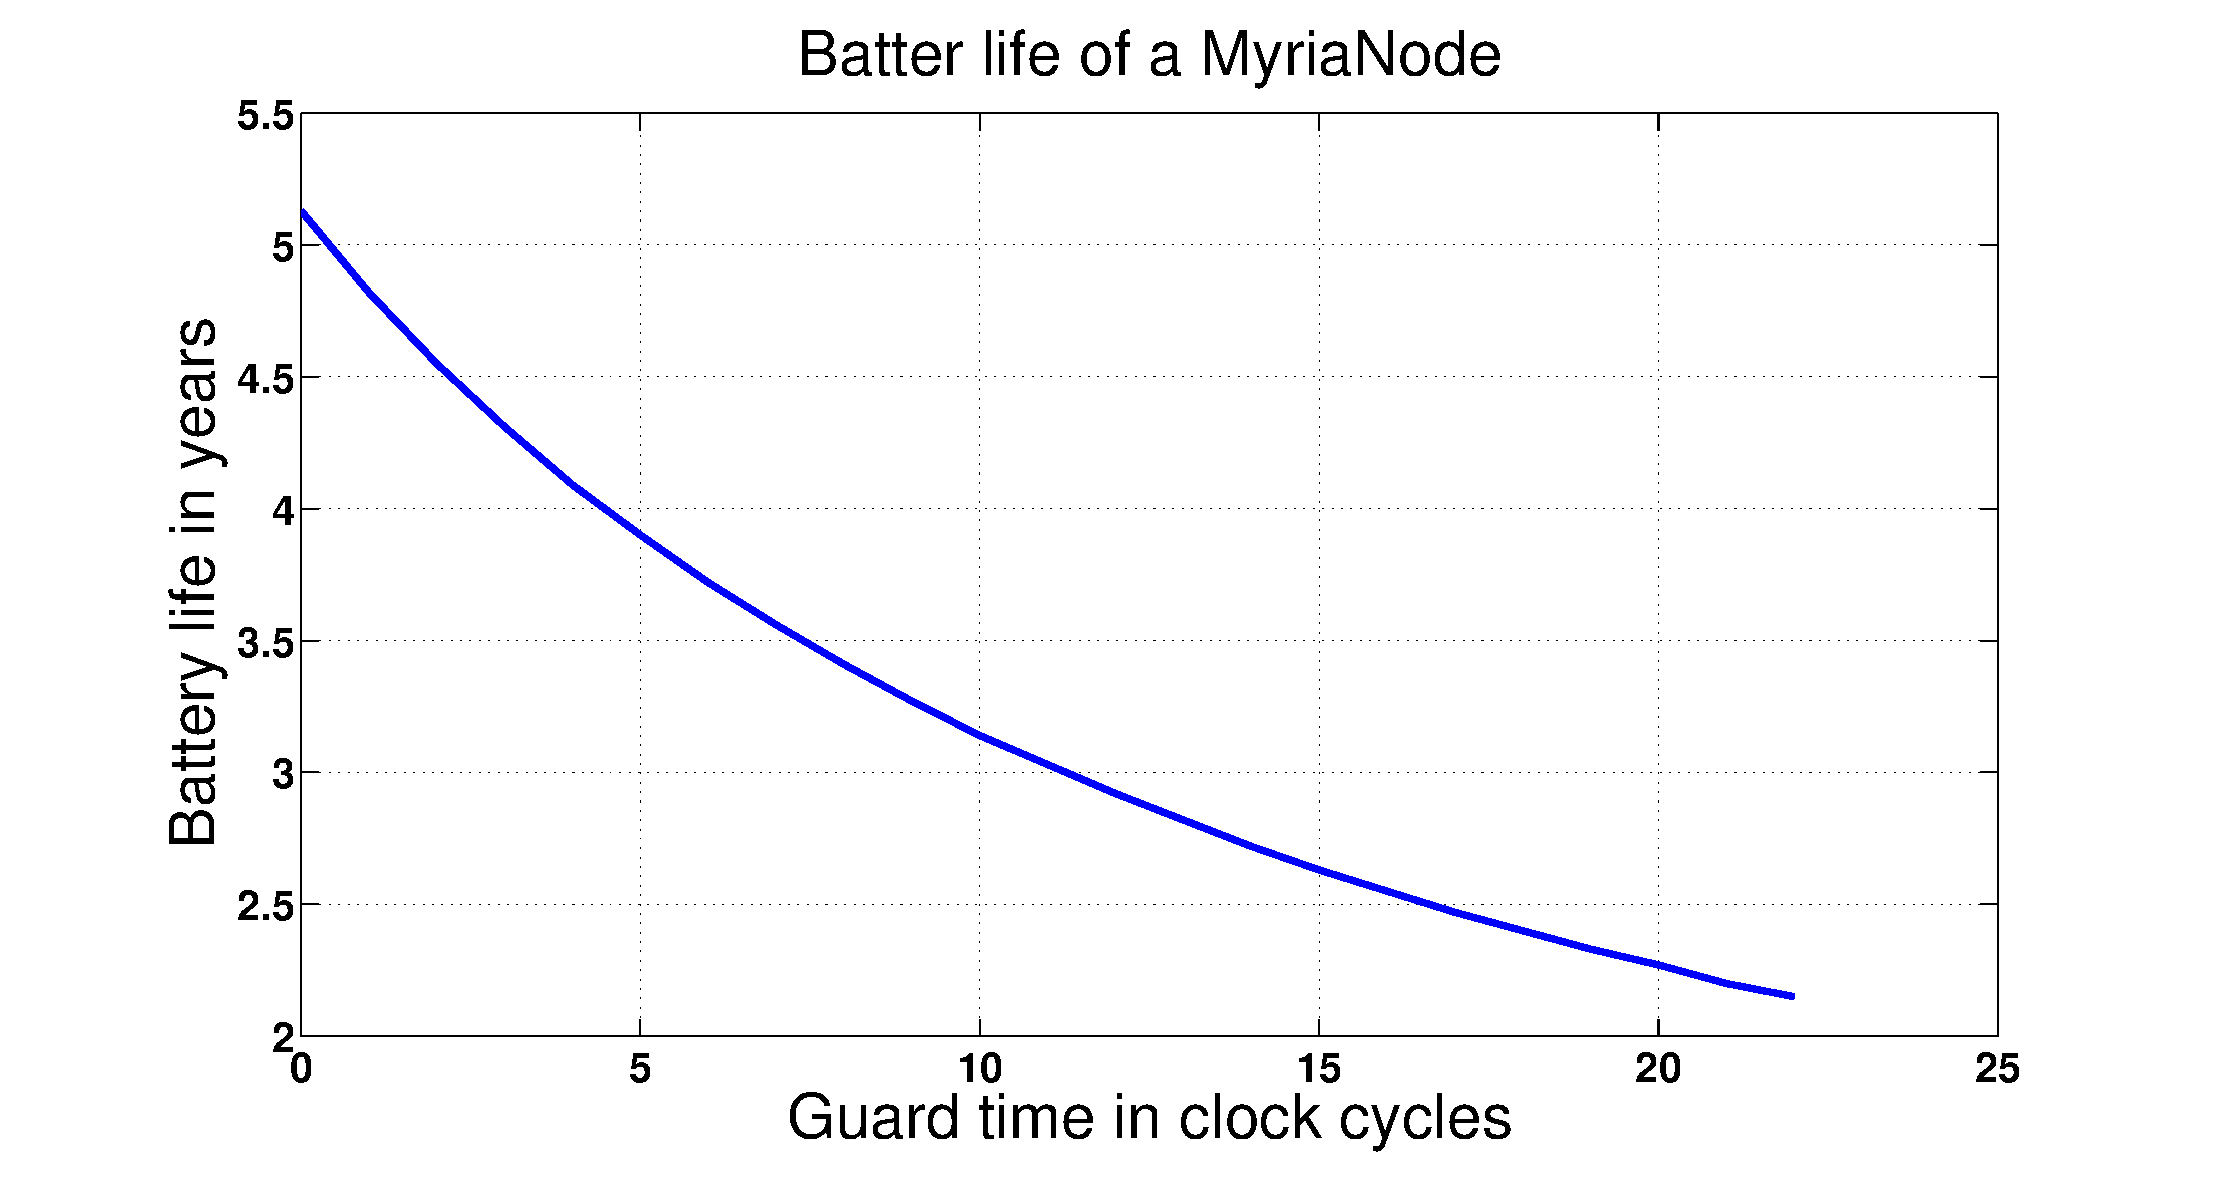
\includegraphics[width=0.5\textwidth]{guardsave}
%\caption{The energy consumption of guard time per RX slot}
%\label{guardsave}
%\end{figure}
\textbf{Additional energy expenditure}\par \noindent
As the results in the previous subsection shows, KF algorithm performs well in all conditions, so do WM and LS when stability is a vital metric. The downside in implementing these algorithms, despite the performance gain achieved, is the energy consumption. As the algorithms are going to be implemented on the sensor nodes, the energy consumption is a priority in embedded system algorithm development. The algorithms are written in C and implemented on the test nodes to see the effect that they are going to have on the energy consumption of the nodes and presented below. \par
The results shown in the table below do not reflect the exact energy consumption of the algorithms as the energy consumption is dependent on other factors besides the execution time. But it can be used to put the comparison into perspective. 
\begin{center}
    \begin{tabular}{ |p{1.5cm} | p{2cm} |p{2cm} |p{1.75cm} | }
    \hline \hline
    Algorithm & Average Execution Time per frame & Increase in execution time per frame & Energy Consumed per frame \\ \hline
    M &  65 $\mu$s & 0 & 0  \\ \hline
    LS & 82.5 $\mu$s & 7.5$\mu$s & 0.063 $\mu J$  \\ \hline
    WM &   90 $\mu$s & 25$\mu$s & 0.21 $\mu J$ \\ \hline
    KF &  150 $\mu$s  & 85$\mu$s &  0.714 $\mu J$\\ \hline
    \end{tabular}
\label{tab}
\end{center}
\textbf{Energy gain}\par \noindent
%As communication costs more than computation[data sheet MyriaNode v2.0], a tradeoff can be done.
In order to reduce the energy that is going to be spent on the algorithm with a better performance, the guard time of the slot can be reduced, due to a better performance showing by KF, WM and LS.
Hence, $t_{guard}$ for KF is taken to be 10$clk$ whereas the guard time for WM and LS is taken to be $24clk$ each from the simulation results. $t_{guard}$ for the Median is taken to be 26$clk$. The number of slots is taken to be 10, so the total guard time per frame will be 10 times $t_{guard}$. In the following table, the energy saving is calculated in comparison with the Median.
\begin{center}
    \begin{tabular}{ |p{1.5cm} | p{2cm} |p{2cm} | p{1.75cm} |  }
    \hline \hline
    Algorithm & Guard time per frame & Reduction in $t_{guard}$ per frame & Energy saving per frame\\ \hline
   M &  792 $\mu$s x 10 & 0 & 0 \\ \hline
    LS & 732 $\mu$s x 10 & 600 $\mu$s & 16.27$\mu J$\\ \hline
    WM &   732 $\mu$s x 10 & 600 $\mu$s & 16.27$\mu J$ \\ \hline
    KF &  305 $\mu$s x 10 & 4870 $\mu$s & 132.07$\mu J$\\ \hline
    \end{tabular}
\end{center}
The length of the guard time has a close-to-linear relation with the power being consumed in listening to the channel. Thus, with the performance gain obtained, the guard time of the slot can be decreased, hereby decreasing the energy consumption of the node in general. Comparing the energy consumption and the energy expenditures, a net gain can be obtained from the proposed algorithms. It can be noted here that communication costs more than computation (as listening radio consumes more energy than CPU active time). Since the length of the guard time is dependent on the number of slots, the energy to be saved increases as the number of slots increases.
\begin{figure}
\centering
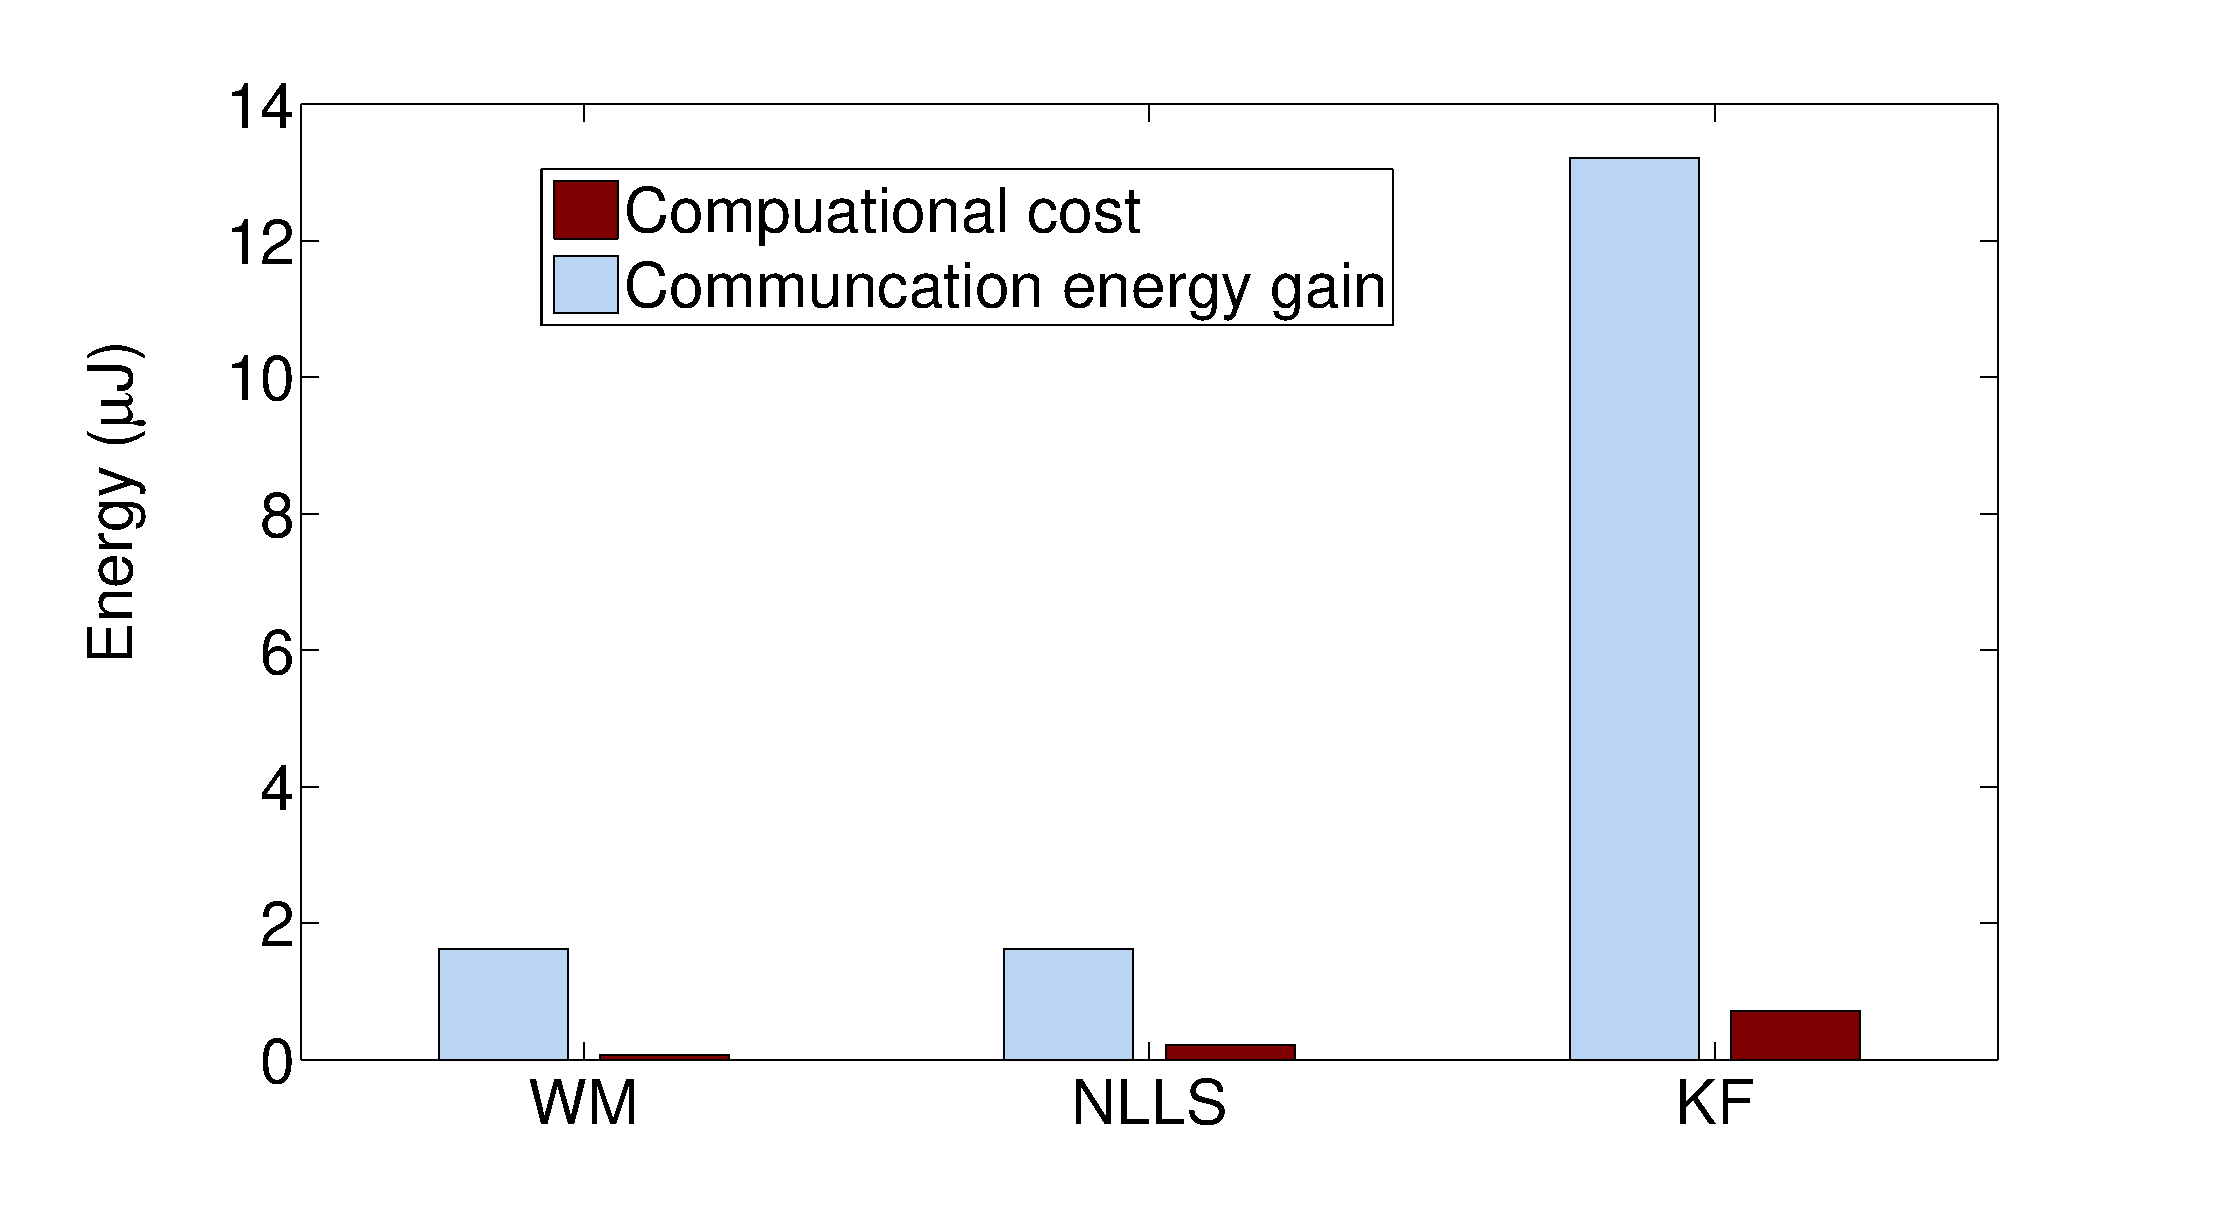
\includegraphics[width=0.5\textwidth]{commvscompute}
\caption{The energy gain of reducing the guard time compared with
the computational cost per RX slot} \label{guardsave}
\end{figure}
\section{\textbf{Conclusion and Recommendation}}\noindent
\textbf{Conclusion}\par
Decentralized synchronization algorithms are proposed for a TDMA-based WSN using Weighted Measurements (WM), Least Squares(LS) and Kalman Filter (KF) methods. Simulation is conducted with different scenarios, especially taking the effect of mobility. Comparison of the algorithms with the currently implemented Median algorithm is conducted and the results are presented.
\par
In a static environment where the nodes are stationary, the KF performs the best whereas the WM and LS have shown a similar performance since they incline to calculate the average of the phase errors. In terms of stability, all the three algorithms have shown a similar performance.
\par
WM and LS show a better tolerance in a dynamic network. Having a
faster adaptation to the changes in the network made the algorithms
preferred ones to a network characterized with dynamic behavior. KF
estimation of the next wake up time is the best with its adaptive feedback nature. KF has also better stability, better
resistant to topology changes occurring in the network.
\par
Using these algorithms for a TDMA-based WSN synchronization (WM, LS and KF), the precision of the synchronization error as well as the stability increases. This in turn has a positive impact on the energy consumption of the nodes because the synchronization period, $T_{sync}$ can be increased or the guard time of the node's frame, $t_{guard}$, can be reduced to achieve the same performance as the Median algorithm. Results are presented and discussed. But in the downside, the energy consumption of the algorithms is greater than the Median algorithm's energy consumption as the algorithms are more complex computationally. Analysis is made and presented about the energy saving made by decreasing the guard time of the slot. Communication is in general more expensive than computation on MyriaNodes, when put into perspective. A net gain of battery life can thus be achieved by using the proposed algorithms.
\par \noindent \textbf{Recommendation} \par Different software power minimization techniques can be applied to further reduce the power consumption of the proposed algorithms, making them more energy efficient for implementation. In addition to that, evaluation and enhancements on the proposed algorithms can be done after implementing them on the MyriaNodes. Real time feedbacks can be used to improve the algorithms towards perfection.
\section{\textbf{Acknowledgment}}This research is part of the MyriaNed$\cite{myrianed}$ Project. The author would like to thank Frits van der Wateren from Chess$\cite{chess}$ Innovation Team for his continuous support, suggestions and advice during the project. Many thanks to dr.ir. Peter Smulders, prof.dr.ir. Erik Fledderus and prof.dr.ir. Peter Baltus from TU\slash e for their guidance.
\begin{thebibliography}{\textbf{References}}
\bibitem{correlation}A.Ebner and et al. "Decentralized Slot Synchronization in Highly Dynamic Ad Hoc Networks," Wireless Personal Multimedia Communications, vol.2, pp.494-498, 2002.
\bibitem{11}C.Cordeiro and D.Agrawal. "Wireless sensor networks", Ad hoc and Sensor Networks Theory and applications. p.429-441. World Scientific Publishing. 2006.
\bibitem{1}F.Zhao and  L.Guibas. "Time synchronization", Wireless Sensor Networks: an Information Processing approach. pp.107-108. Elsevier. 2004.
\bibitem{taxonomy}E.Anceaume and I.Puaut. "A taxonomy of clock synchronization algorithms". IRISA Research Report No. PI1103, IRISA, 1997.\bibitem{10}H.Karl and A.Willig. "Introduction" in Protocols and Architectures for Wireless Sensor Networks. pp. 3-6. Wiley. July 2006.
\bibitem{clockwhite}Symmetricom, Inc. white paper. "Stochastic Model Estimation of network time variance," USA.2004.
\bibitem{19}Dallas semiconductor."Crystal considerations with Dallas Real time clocks," Available online http:\slash \slash pdfserv.maxim-ic.com\slash en\slash an\slash AN58.pdf [Accessed on July 15,2008].
\bibitem{18}Golledge frequency products."SW Watch crystal temp mil," Available online http:\slash \slash www.golledge.co.uk\slash pdf\slash products\slash xtl$\_$sm\slash cc7v.pdf [Accessed on July 15,2008].
\bibitem{kalm}G.Welch and G.Bishop. "The kalman filter," University of North Carolina. Avalable online http:\slash \slash www.cs.unc.edu\slash ~welch\slash kalman\slash  [Accessed on June 10, 2008].
\bibitem{2}J.Elson, L.Girod and D.Estrin. "Fine-grained network time synchronization using reference broadcasts," Proceedings of the 5th Symposium on Operating Systems Design and Implementation, Vol.36 , Issue SI, pp.147-163, 2002.
\bibitem{pieter}P.Anemaet. Determining G-MAC potential with $\{$S,L,SCP$\}$-MAC. Masters thesis. Technische Universteit Delft. Delft. August 2008.
\bibitem{3}Q.Yang, and et al. "A Decentralized Slot Synchronization Algorithm for TDMA-Based Ad Hoc Networks," Wireless Communications, Networking and Mobile Computing, Vol., Issue,21-25, pp. 1717-1721, 2007.
\bibitem{17}Q.Yang and J.Shi. "An interference elimination method for decentralized slot synchronization in TDMA-based wireless ad hoc network," Intelligent Signal Processing and Communication Systems, pp 236-239, 2007.
\bibitem{median}R.Tjoa and et al. "Clock drift reduction for relative time slot tdma-based sensor networks," Personal, Indoor and Mobile Radio Communications, Vol.2, 5-8 , pp.1042-1047. Sept. 2004.
\bibitem{6}R.John. "Introduction to Quartz Frequency Standards," Technical Report SLCET-TR-92-1, Army Research Laboratory, Electronics and Power Sources Directorate. October 1992.
%\bibitem{7}J.Elson and D.Estrin. Time Synchronization for Wireless Sensor Networks. In Proceedings of the 15th International Parallel and Distributed Processing Symposium. IEEE Computer Society, April 23-27. 2001.
%\bibitem{9}K.Romer. Time Synchronization in Ad Hoc Networks. In Proceedings of the Second ACM International Symposium on Mobile Ad Hoc Networking and Computing, Long Beach, California. 2001.
\bibitem{texas}S.Raje and Q.Liang. "Time synchronization of in Network-centric sensor networks," Radio and Wireless Symposium IEEE, pp.333-336. 2007.
\bibitem{myrianed}MyrianNed project. "Project description," Available online. http:\slash \slash www.chess.nl\slash en\slash home\slash Innovatie\slash Onderzoek\slash MyriaNed [Accessed on August 3, 2008].
\bibitem{chess}Company profile. Available online http://www.chess.nl [Accessed on August 6, 2008].
%\bibitem{14}S.PalChaudhuri and et al. "Adaptive Clock Synchronization in Sensor Networks," Information Processing in Sensor Networks, pp.340-348, 2004.
%\bibitem{16}G.Werner-Allen and et al. Firefly-inspired sensor network synchronicity with realistic radio effects. Proceedings of the 3rd international conference on Embedded networked sensor systems, San Diego, California. November 2005.
\end{thebibliography}
\end{document}
